%%%%%%%%%%%%%%%%%%%%%%%%%%%%%%%%%%%%%%%%%
% Programming/Coding Assignment
% LaTeX Template
%
% This template has been downloaded from:
% http://www.latextemplates.com
%
% Original author:
% Ted Pavlic (http://www.tedpavlic.com)
%
% Note:
% The \lipsum[#] commands throughout this template generate dummy text
% to fill the template out. These commands should all be removed when 
% writing assignment content.
%
% This template uses a Perl script as an example snippet of code, most other
% languages are also usable. Configure them in the "CODE INCLUSION 
% CONFIGURATION" section.
%
%%%%%%%%%%%%%%%%%%%%%%%%%%%%%%%%%%%%%%%%%

%----------------------------------------------------------------------------------------
%	PACKAGES AND OTHER DOCUMENT CONFIGURATIONS
%----------------------------------------------------------------------------------------

\documentclass{article}

\usepackage{fancyhdr} % Required for custom headers
\usepackage{lastpage} % Required to determine the last page for the footer
\usepackage{extramarks} % Required for headers and footers
\usepackage[usenames,dvipsnames]{color} % Required for custom colors
\usepackage{graphicx} % Required to insert images
\usepackage{listings} % Required for insertion of code
\usepackage{courier} % Required for the courier font
\usepackage{lipsum} % Used for inserting dummy 'Lorem ipsum' text into the template
\usepackage{setspace}
\usepackage{color}
\usepackage{comment}
\usepackage{caption}

\usepackage{hyperref}
\usepackage{natbib}
\usepackage{underscore}
\usepackage{subfigure}


\hypersetup{
    colorlinks=true,
    linkcolor=blue,
    filecolor=magenta,      
    urlcolor=cyan,
    breaklinks=true
}

%\usepackage[]{algorithm2e}
\usepackage{pdfpages}




%For python inclusion (http://widerin.org/blog/syntax-highlighting-for-python-scripts-in-latex-documents)
\definecolor{Code}{rgb}{0,0,0}
\definecolor{Decorators}{rgb}{0.5,0.5,0.5}
\definecolor{Numbers}{rgb}{0.5,0,0}
\definecolor{MatchingBrackets}{rgb}{0.25,0.5,0.5}
\definecolor{Keywords}{rgb}{0,0,1}
\definecolor{self}{rgb}{0,0,0}
\definecolor{Strings}{rgb}{0,0.63,0}
\definecolor{Comments}{rgb}{0,0.63,1}
\definecolor{Backquotes}{rgb}{0,0,0}
\definecolor{Classname}{rgb}{0,0,0}
\definecolor{FunctionName}{rgb}{0,0,0}
\definecolor{Operators}{rgb}{0,0,0}
\definecolor{Background}{rgb}{0.98,0.98,0.98}

% Margins
\topmargin=-0.45in
\evensidemargin=0in
\oddsidemargin=0in
\textwidth=6.5in
\textheight=9.0in
\headsep=0.25in

\linespread{1.1} % Line spacing

% Set up the header and footer
\pagestyle{fancy}
\lhead{\hmwkAuthorName} % Top left header
%\chead{\hmwkClass\ (\hmwkClassInstructor\ \hmwkClassTime): \hmwkTitle} % Top center head
\chead{\hmwkClass\ (\hmwkClassInstructor): \hmwkTitle} % Top center head
\rhead{\firstxmark} % Top right header
\lfoot{\lastxmark} % Bottom left footer
\cfoot{} % Bottom center footer
\rfoot{Page\ \thepage\ of\ \protect\pageref{LastPage}} % Bottom right footer
\renewcommand\headrulewidth{0.4pt} % Size of the header rule
\renewcommand\footrulewidth{0.4pt} % Size of the footer rule

\setlength\parindent{0pt} % Removes all indentation from paragraphs

%----------------------------------------------------------------------------------------
%	CODE INCLUSION CONFIGURATION
%----------------------------------------------------------------------------------------

\definecolor{MyDarkGreen}{rgb}{0.0,0.4,0.0} % This is the color used for comments
\lstloadlanguages{Perl} % Load Perl syntax for listings, for a list of other languages supported see: ftp://ftp.tex.ac.uk/tex-archive/macros/latex/contrib/listings/listings.pdf
\lstset{language=Perl, % Use Perl in this example
        frame=single, % Single frame around code
        basicstyle=\small\ttfamily, % Use small true type font
        keywordstyle=[1]\color{Blue}\bf, % Perl functions bold and blue
        keywordstyle=[2]\color{Purple}, % Perl function arguments purple
        keywordstyle=[3]\color{Blue}\underbar, % Custom functions underlined and blue
        identifierstyle=, % Nothing special about identifiers                                         
        commentstyle=\usefont{T1}{pcr}{m}{sl}\color{MyDarkGreen}\small, % Comments small dark green courier font
        stringstyle=\color{Purple}, % Strings are purple
        showstringspaces=false, % Don't put marks in string spaces
        tabsize=5, % 5 spaces per tab
        %
        % Put standard Perl functions not included in the default language here
        morekeywords={rand},
        %
        % Put Perl function parameters here
        morekeywords=[2]{on, off, interp},
        %
        % Put user defined functions here
        morekeywords=[3]{test},
       	%
        morecomment=[l][\color{Blue}]{...}, % Line continuation (...) like blue comment
        numbers=left, % Line numbers on left
        firstnumber=1, % Line numbers start with line 1
        numberstyle=\tiny\color{Blue}, % Line numbers are blue and small
        stepnumber=5 % Line numbers go in steps of 5
}

% Creates a new command to include a perl script, the first parameter is the filename of the script (without .pl), the second parameter is the caption
\newcommand{\perlscript}[2]{
\begin{itemize}
\item[]\lstinputlisting[caption=#2,label=#1]{#1.pl}
\end{itemize}
}


%----------------------------------------------------------------------------------------
%	DOCUMENT STRUCTURE COMMANDS
%	Skip this unless you know what you're doing
%----------------------------------------------------------------------------------------

% Header and footer for when a page split occurs within a problem environment
\newcommand{\enterProblemHeader}[1]{
\nobreak\extramarks{#1}{#1 continued on next page\ldots}\nobreak
\nobreak\extramarks{#1 (continued)}{#1 continued on next page\ldots}\nobreak
}

% Header and footer for when a page split occurs between problem environments
\newcommand{\exitProblemHeader}[1]{
\nobreak\extramarks{#1 (continued)}{#1 continued on next page\ldots}\nobreak
\nobreak\extramarks{#1}{}\nobreak
}

\setcounter{secnumdepth}{0} % Removes default section numbers
\newcounter{homeworkProblemCounter} % Creates a counter to keep track of the number of problems

\newcommand{\homeworkProblemName}{}
\newenvironment{homeworkProblem}[1][Problem \arabic{homeworkProblemCounter}]{ % Makes a new environment called homeworkProblem which takes 1 argument (custom name) but the default is "Problem #"
\stepcounter{homeworkProblemCounter} % Increase counter for number of problems
\renewcommand{\homeworkProblemName}{#1} % Assign \homeworkProblemName the name of the problem
\section{\homeworkProblemName} % Make a section in the document with the custom problem count
\enterProblemHeader{\homeworkProblemName} % Header and footer within the environment
}{
\exitProblemHeader{\homeworkProblemName} % Header and footer after the environment
}

\newcommand{\problemAnswer}[1]{ % Defines the problem answer command with the content as the only argument
\noindent\framebox[\columnwidth][c]{\begin{minipage}{0.98\columnwidth}#1\end{minipage}} % Makes the box around the problem answer and puts the content inside
}

\newcommand{\homeworkSectionName}{}
\newenvironment{homeworkSection}[1]{ % New environment for sections within homework problems, takes 1 argument - the name of the section
\renewcommand{\homeworkSectionName}{#1} % Assign \homeworkSectionName to the name of the section from the environment argument
\subsection{\homeworkSectionName} % Make a subsection with the custom name of the subsection
\enterProblemHeader{\homeworkProblemName\ [\homeworkSectionName]} % Header and footer within the environment
}{
\enterProblemHeader{\homeworkProblemName} % Header and footer after the environment
}

%----------------------------------------------------------------------------------------
%	NAME AND CLASS SECTION
%----------------------------------------------------------------------------------------

\newcommand{\hmwkTitle}{Assignment\ \#6 } % Assignment title
%\newcommand{\hmwkDueDate}{Monday,\ January\ 1,\ 2012} % Due date
\newcommand{\hmwkClass}{Introduction to Web Science} % Course/class
%\newcommand{\hmwkClassTime}{10:30am} % Class/lecture time
\newcommand{\hmwkClassInstructor}{Dr. Nelson} % Teacher/lecturer
\newcommand{\hmwkAuthorName}{Alexander Nwala} % Your name

%----------------------------------------------------------------------------------------
%	TITLE PAGE
%----------------------------------------------------------------------------------------

\title{
\vspace{2in}
\textmd{\textbf{\hmwkClass:\ \hmwkTitle}}\\
%\normalsize\vspace{0.1in}\small{Due\ on\ \hmwkDueDate}\\
%\vspace{0.1in}\large{\textit{\hmwkClassInstructor\ \hmwkClassTime}}
\vspace{0.1in}\large{\textit{\hmwkClassInstructor}}
\vspace{3in}
}

\author{\textbf{\hmwkAuthorName}}
\date{Thursday, October 30, 2014} % Insert date here if you want it to appear below your name

%----------------------------------------------------------------------------------------

\begin{document}

\maketitle



%----------------------------------------------------------------------------------------
%	TABLE OF CONTENTS
%----------------------------------------------------------------------------------------

%\setcounter{tocdepth}{1} % Uncomment this line if you don't want subsections listed in the ToC

\newpage
\tableofcontents
\newpage

%----------------------------------------------------------------------------------------
%	PROBLEM 1
%----------------------------------------------------------------------------------------

% To have just one problem per page, simply put a \clearpage after each problem

\begin{homeworkProblem}

We know the result of the Karate Club (Zachary, 1977) split (Figure 1b).
Prove or disprove that the result of split could have been predicted
by the weighted graph of social interactions.  How well does the
mathematical model represent reality?\\

Generously document your answer with all supporting equations, code,
graphs, arguments, etc.\\

Useful sources include:\\

\textbf{Original paper}
    \begin{verbatim}
    http://aris.ss.uci.edu/~lin/76.pdf
    \end{verbatim}
\textbf{Slides}
    \begin{verbatim}
    http://www-personal.umich.edu/~ladamic/courses/networks/si614w06/ppt/le
    cture18.ppt

    http://clair.si.umich.edu/si767/papers/Week03/Community/CommunityDetect
    ion.pptx
    \end{verbatim}
\textbf{Code and data}
    \begin{verbatim}
    http://networkx.github.io/documentation/latest/examples/graph/karate_cl
    ub.html

    http://nbviewer.ipython.org/url/courses.cit.cornell.edu/info6010/resour
    ces/11notes.ipynb

    http://stackoverflow.com/questions/9471906/what-are-the-differences-bet
    ween-community-detection-algorithms-in-igraph/9478989#9478989

    http://stackoverflow.com/questions/5822265/are-there-implementations-of
    -algorithms-for-community-detection-in-graphs

    http://konect.uni-koblenz.de/networks/ucidata-zachary

    http://vlado.fmf.uni-lj.si/pub/networks/data/ucinet/ucidata.htm#zachary
    \end{verbatim}

\begin{figure}
\caption{Zachary's Karate Club Graphs}

\subfigure[Original Graph]{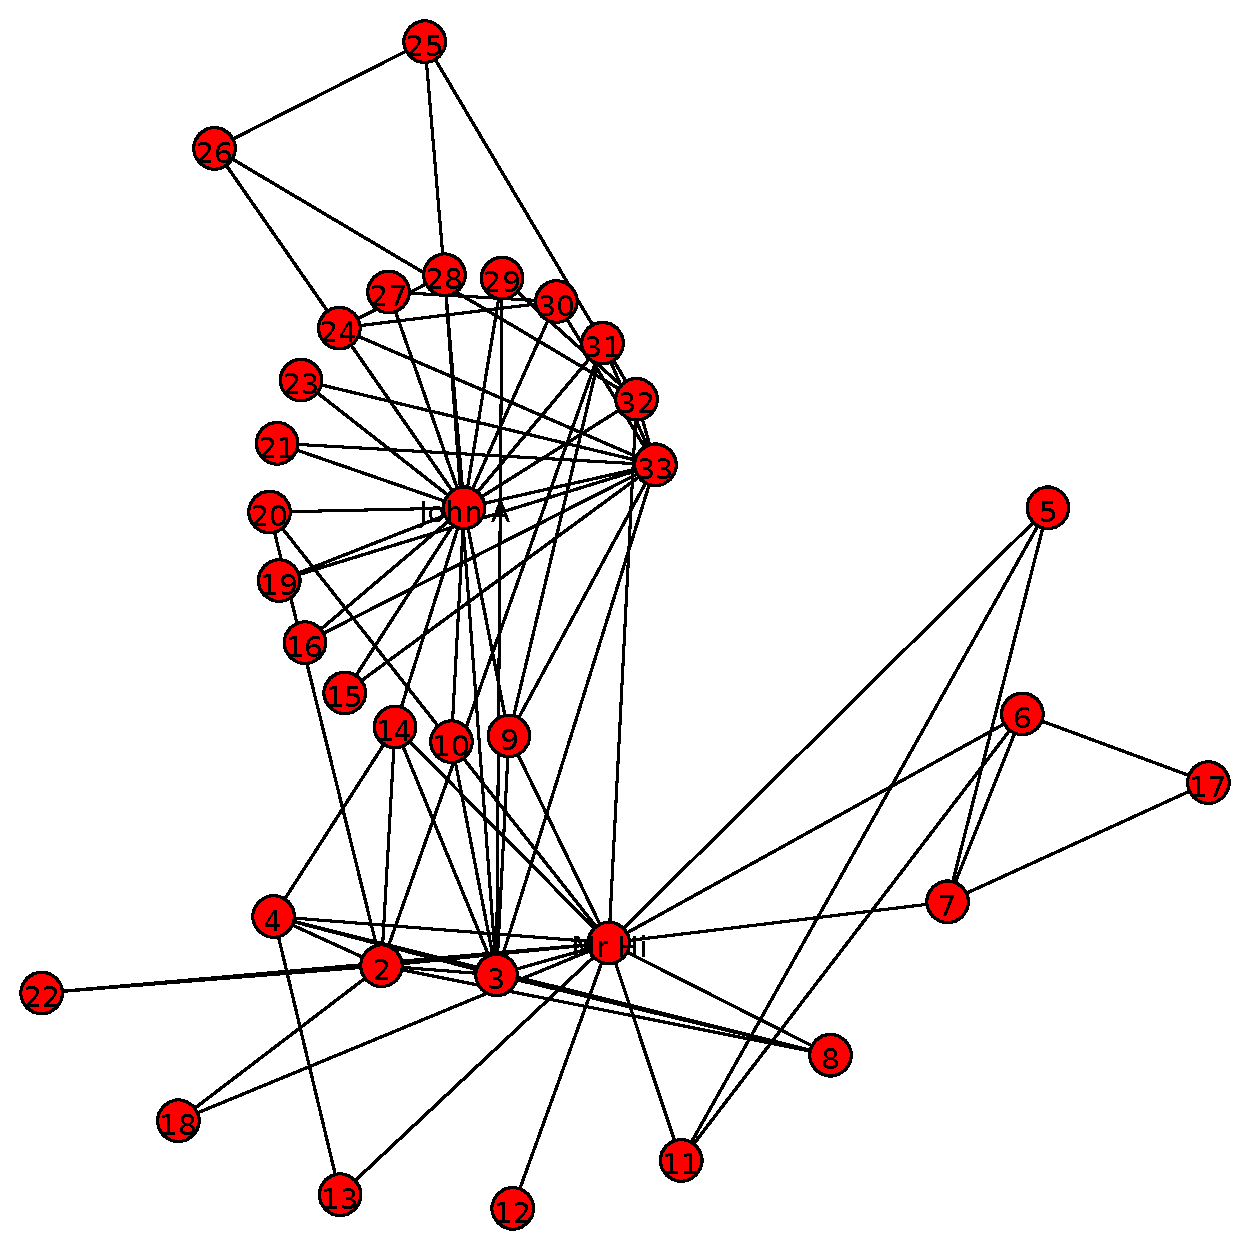
\includegraphics[width=.50\textwidth]{../graphs/originalGraph.pdf}}
\subfigure[Result of Split Graph]{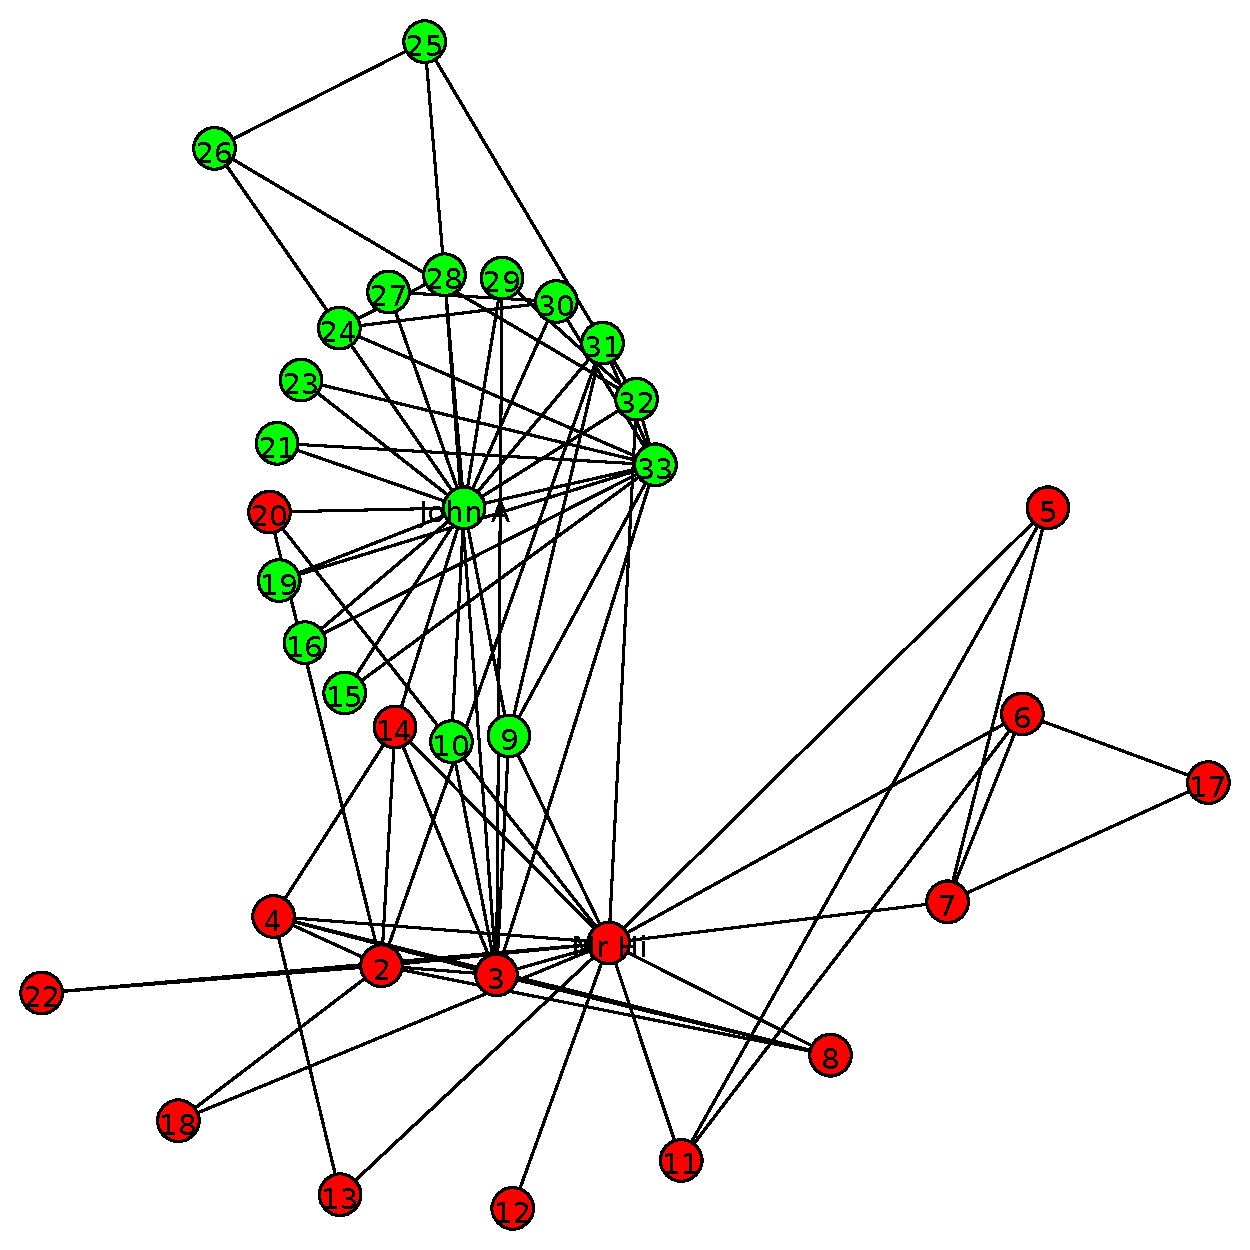
\includegraphics[width=.50\textwidth]{../graphs/factionsGraph.pdf}}

\end{figure}

\begin{comment}
\begin{figure}
    \caption{curlDemoOutput}
    \begin{center}
        \includegraphics{curlDemo} % Example image
    \end{center}
\end{figure}
\end{comment}

%\problemAnswer
%{
    \begin{verbatim}\end{verbatim}
    \textbf{SOLUTION 1}\\

    The strategy I employed in order to prove the result of the split (\textbf{Figure 1b}) is based upon the following rationale:
    Given the Karate Club graph, unity could be attributed to a single important node. However, if importance is split among more than one node, the consequence of this could be disunity or split. This means we should expect to see multiple clusters as opposed to a single cluster.\\

    The mathematical model which mirrors my rationale is the concept of centrality (indicates the most important nodes in a graph). I used the edge betweenness centrality measure in order to measure the centrality. Finally in order to prove the result of the split, I applied the Girvin-Newman algorithm to incrementally see if I could derive the resultant split beginning from the original (non-split) graph (\textbf{Figure 1a}). The idea behind using the Girvin-Newman algorithm is, initially, there is unity (1 cluster in the network), then we seek to look for factions or communities in the network by continuously calculating the betweenness and removing the edge with the highest betweenness.\\

    \begin{verbatim}
        The file karate.GraphML contains the karate club graph
    \end{verbatim}

    The following is a summary of the Girvin-Newman Algorithm I implemented using igraph \cite{igraph} :

    \begin{verbatim}
    Given graph G,
    while( edgeCount > 0 and clusterCount < maximumClusterThreshold )
    {
        allEdgesBetweennessList = G.getBetweennessValues()
        maximumBetweennessValue = getMaximum(allEdgeBetweennessList)

        edgeWithMaximumBetweennessValue = 
        getEgdeWithMaximumBetweennessValue(maximumBetweennessValue)

        G.remove(edgeWithMaximumBetweennessValue)
    }
    \end{verbatim}

    Listing 1 is an outline of the implementation
    \lstinputlisting[breaklines=true, caption=Girvin-Newman Algorithm]{GNA.py}


    \begin{figure}

        \caption{Multiple Iterations Of The Girvin-Newman Algorithm}
        \subfigure[Iteration: 0, Clusters: 1]{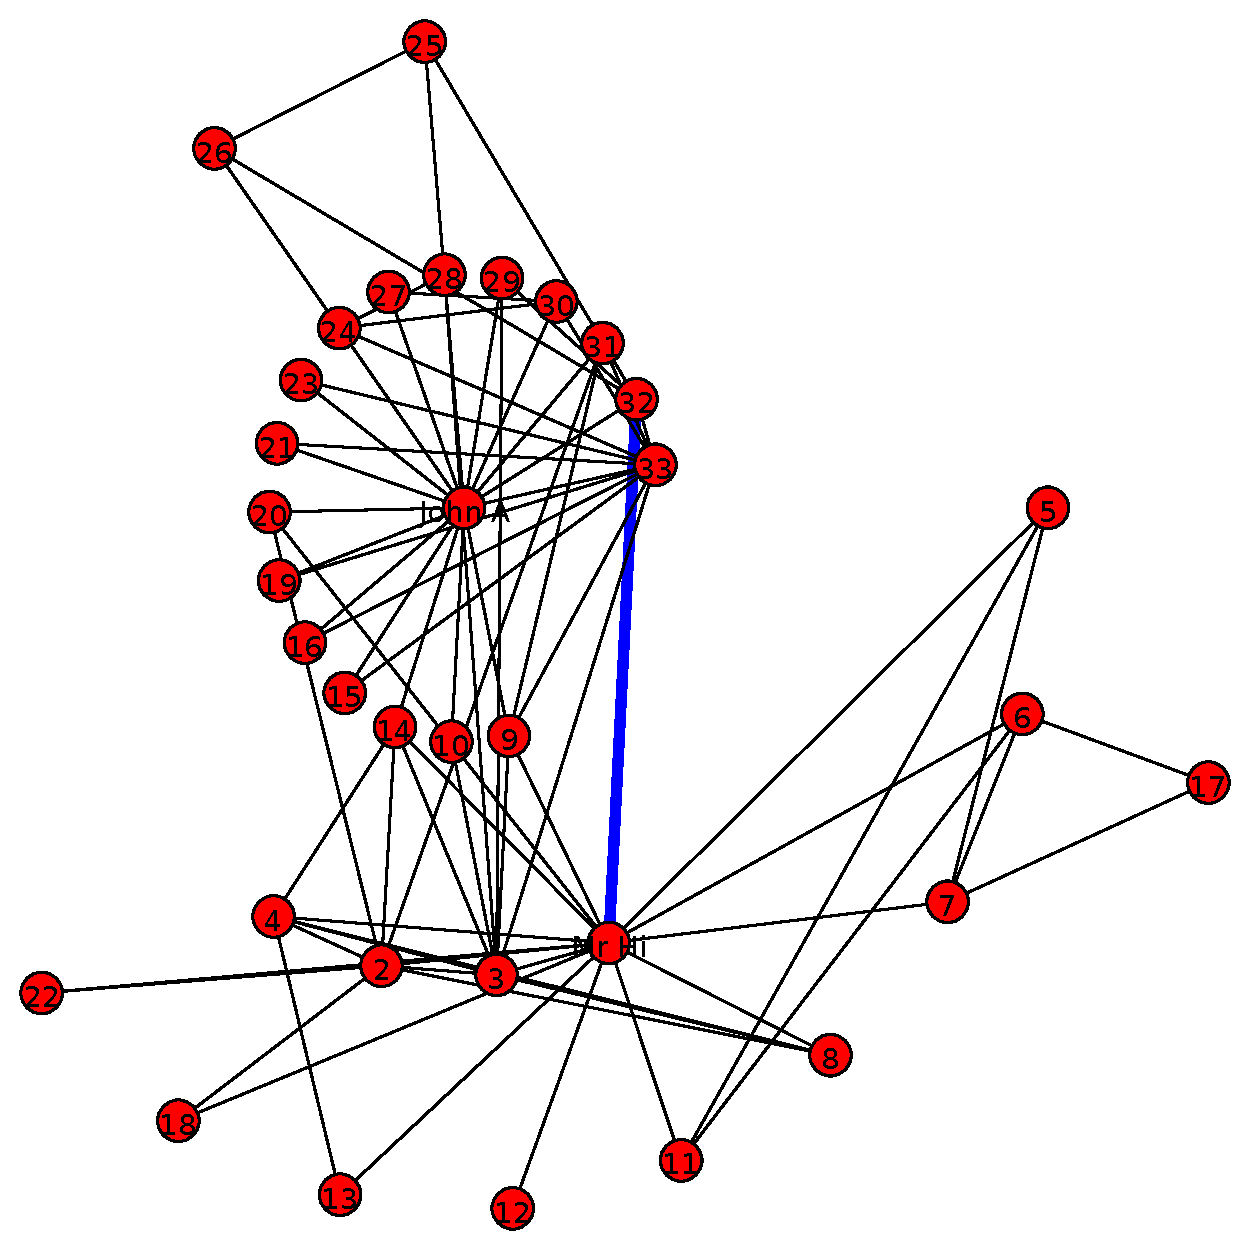
\includegraphics[width=.50\textwidth]{../graphs/sn-0-1.pdf}}
        \subfigure[Iteration: 1, Clusters: 1]{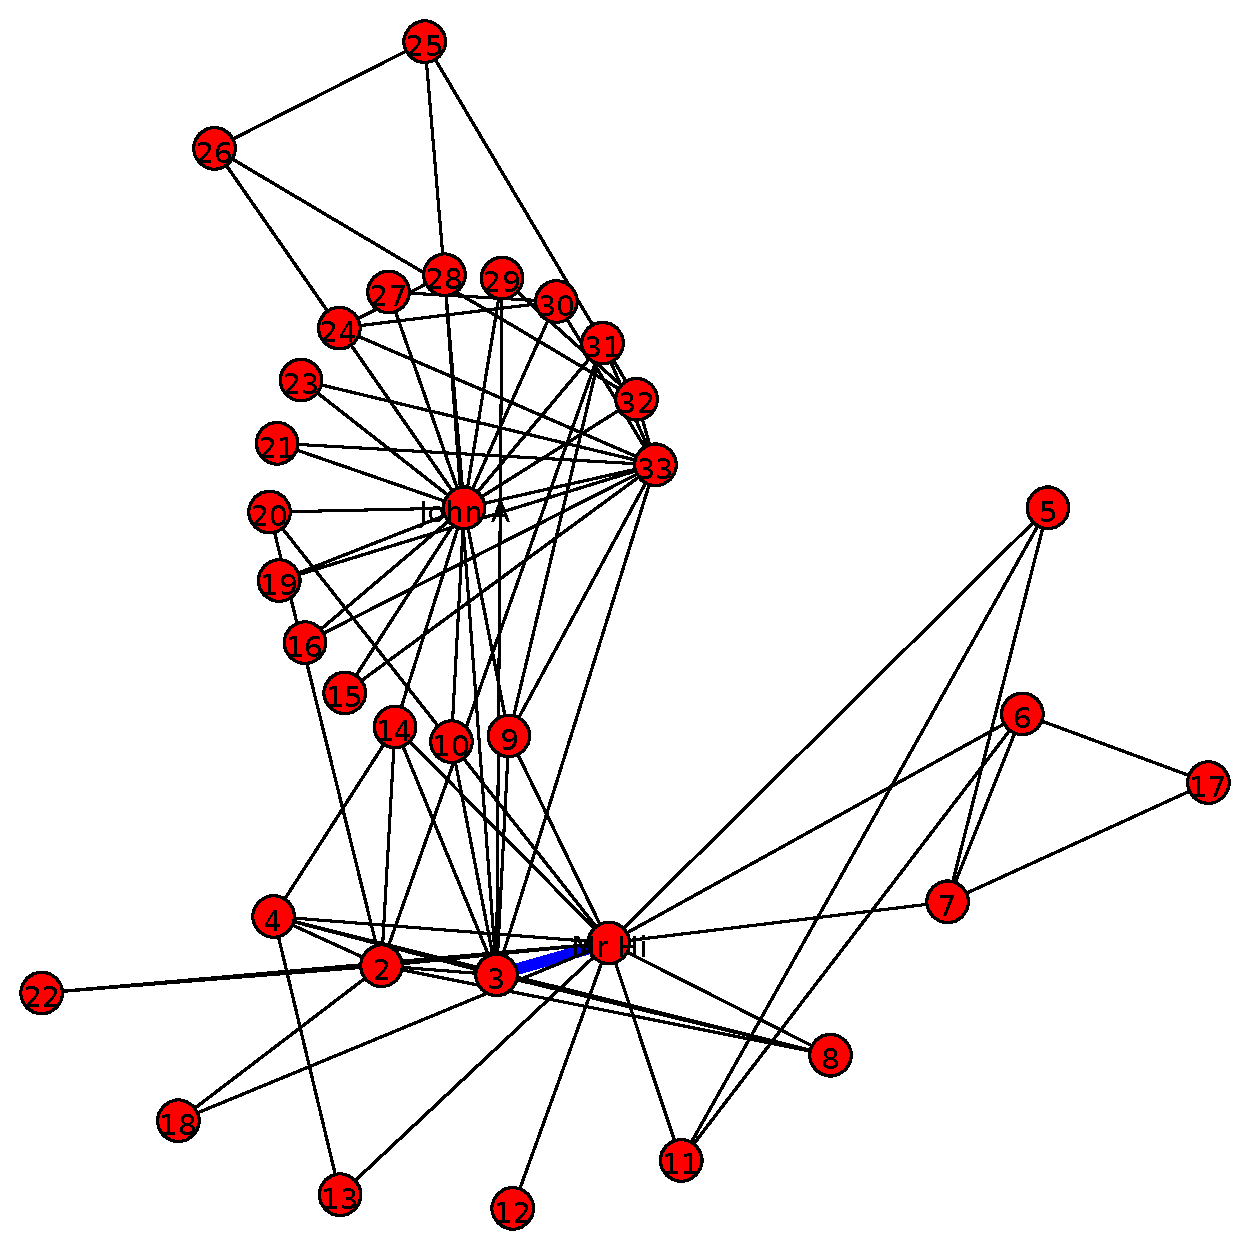
\includegraphics[width=.50\textwidth]{../graphs/sn-1-1.pdf}}
        \subfigure[Iteration: 2, Clusters: 1]{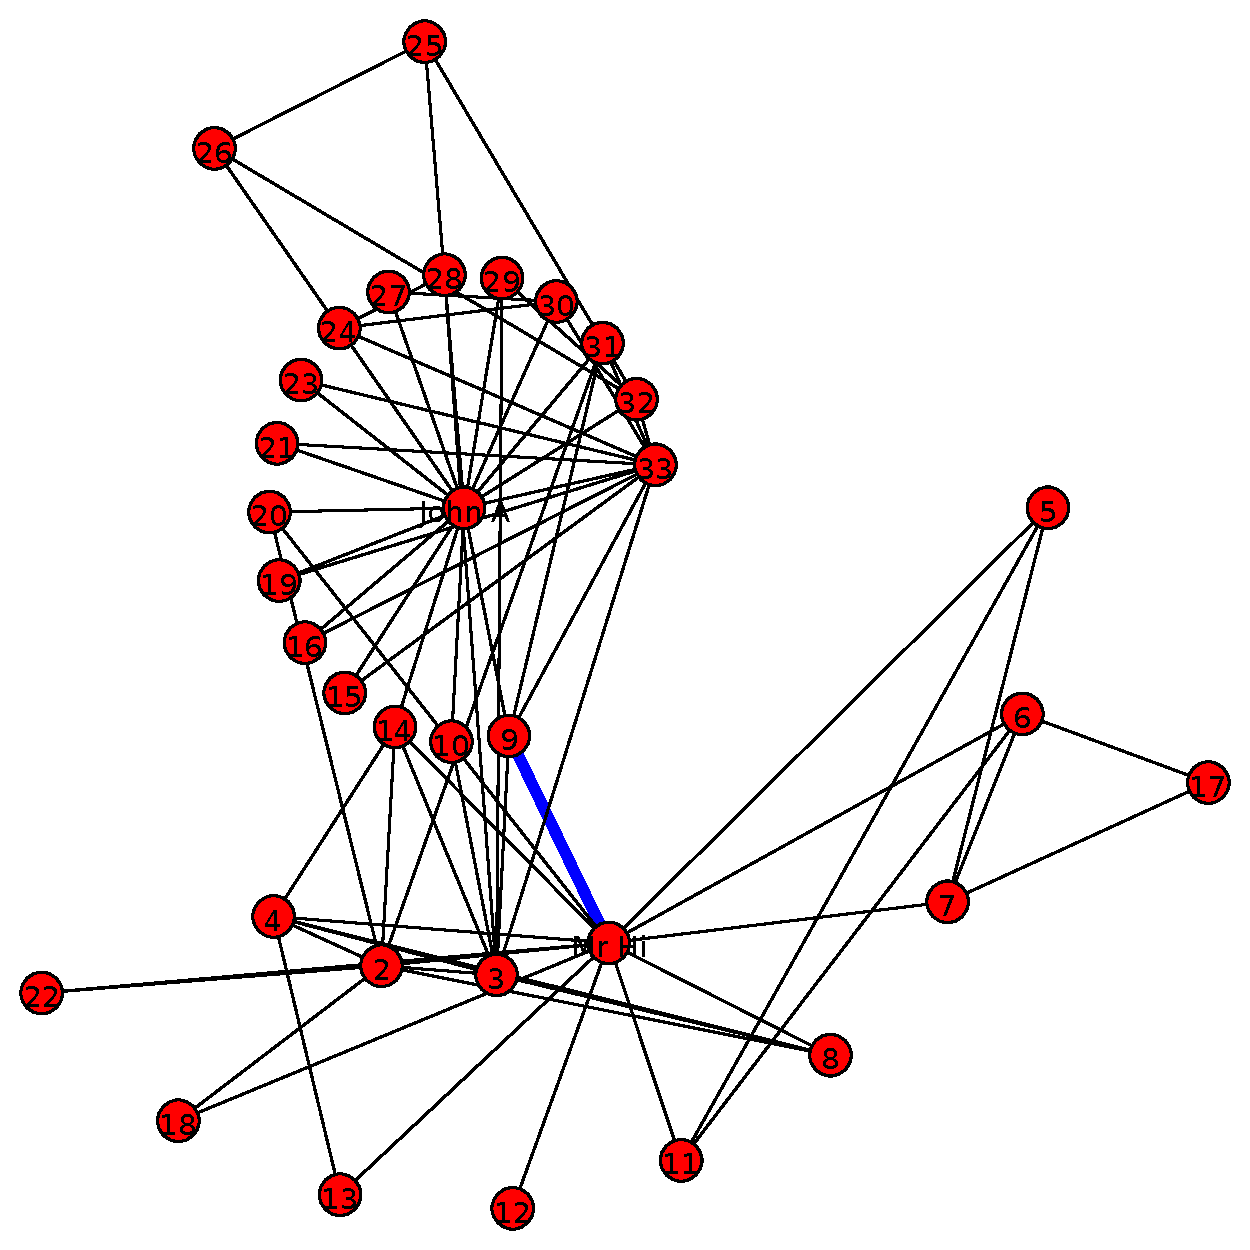
\includegraphics[width=.50\textwidth]{../graphs/sn-2-1.pdf}}
        \subfigure[Iteration: 3, Clusters: 1]{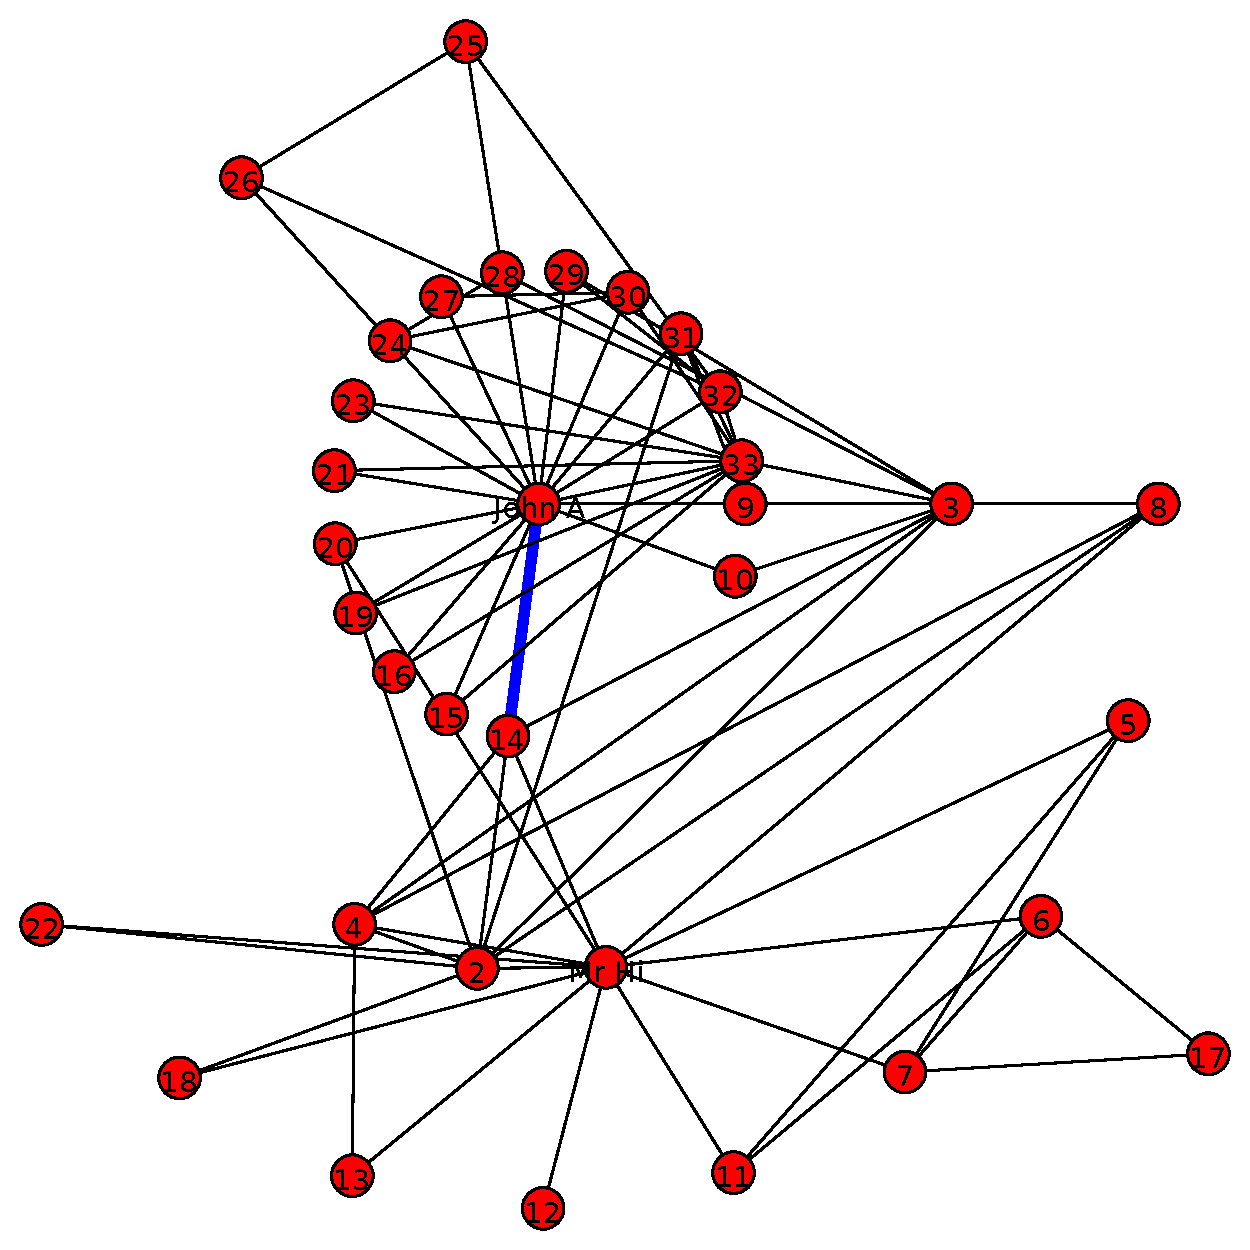
\includegraphics[width=.50\textwidth]{../graphs/sn-3-1.pdf}}

    \end{figure}

    \begin{figure}
    
        \caption{Multiple Iterations Of The Girvin-Newman Algorithm}
        \subfigure[Iteration: 4, Clusters: 1]{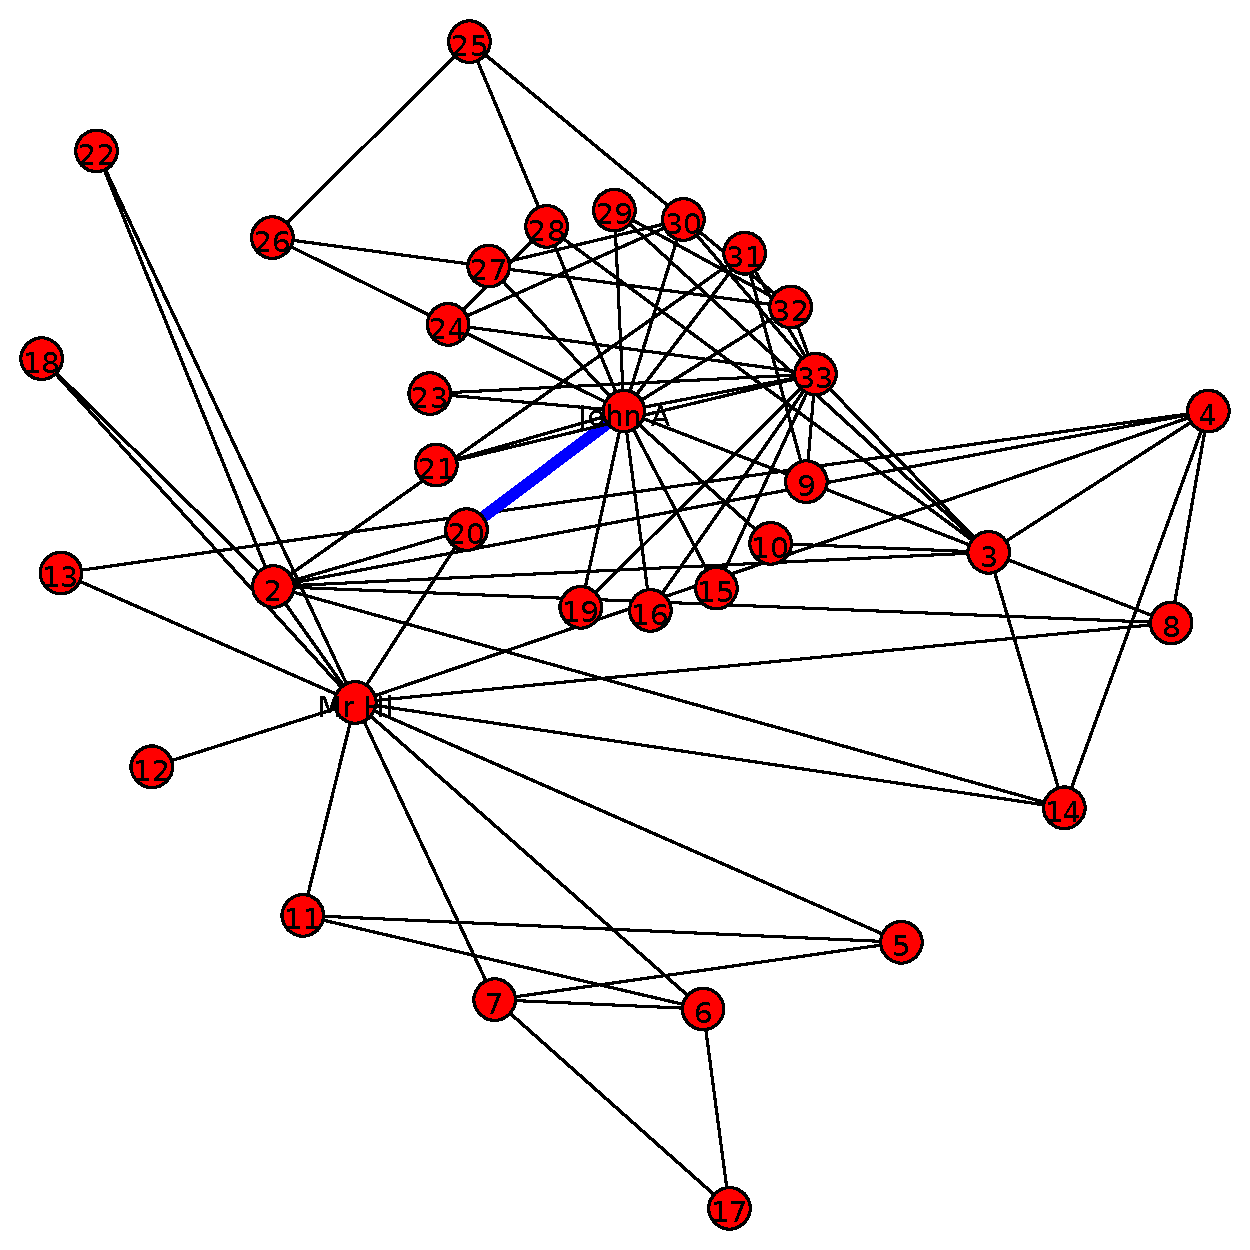
\includegraphics[width=.50\textwidth]{../graphs/sn-4-1.pdf}}
        \subfigure[Iteration: 5, Clusters: 1]{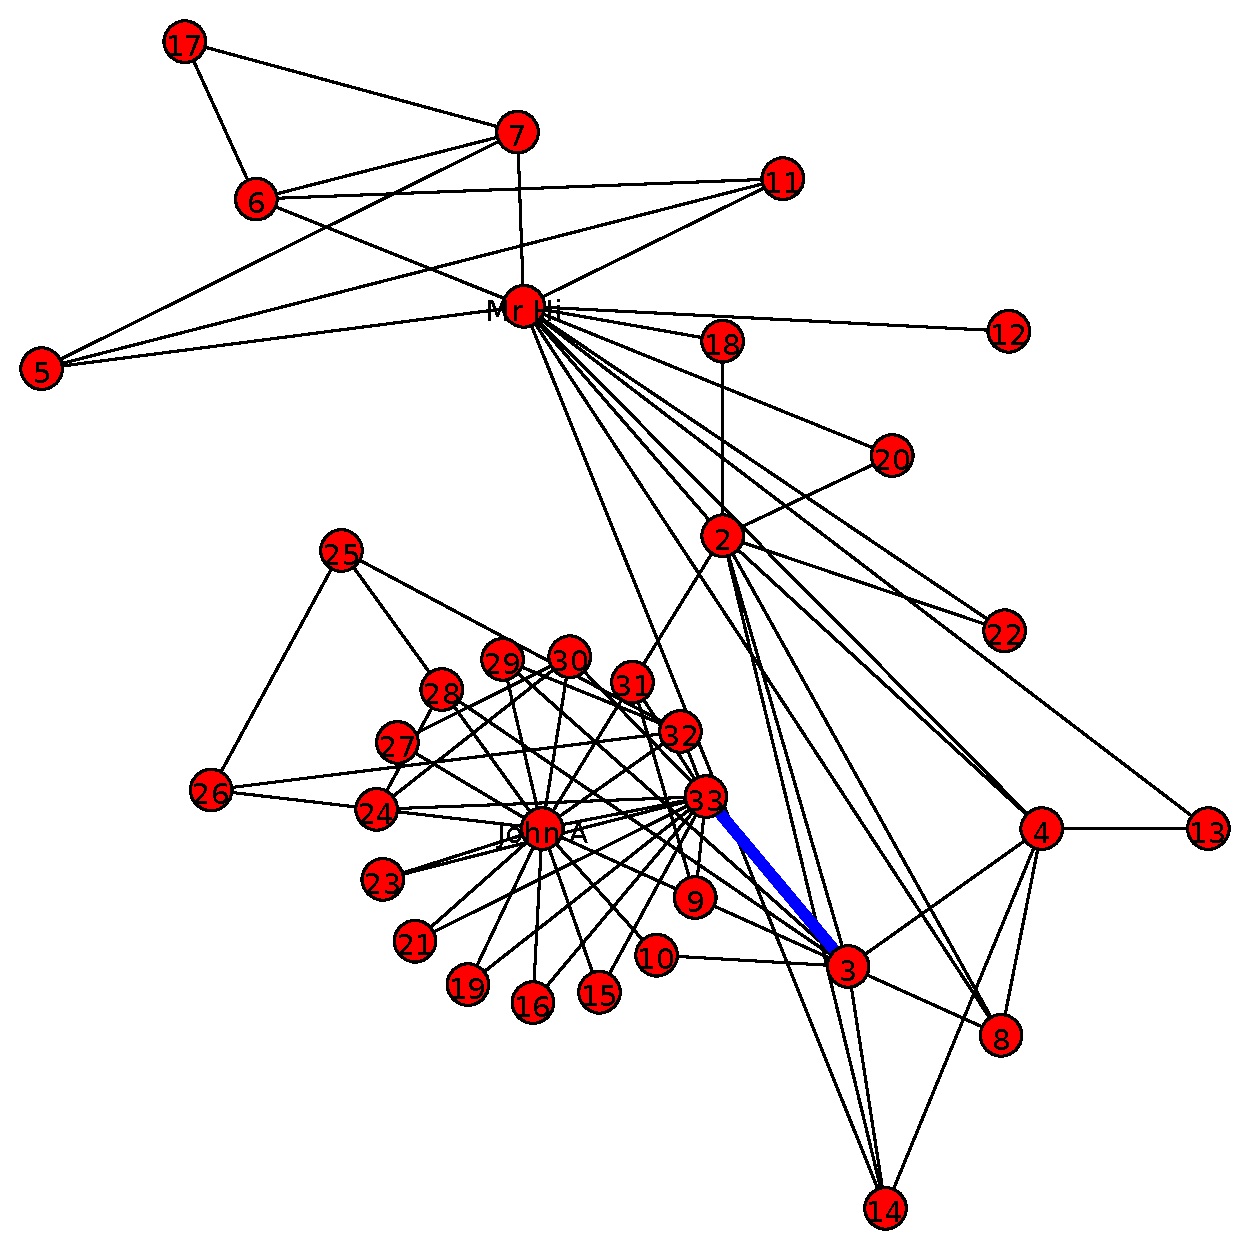
\includegraphics[width=.50\textwidth]{../graphs/sn-5-1.pdf}}
        \subfigure[Iteration: 6, Clusters: 1]{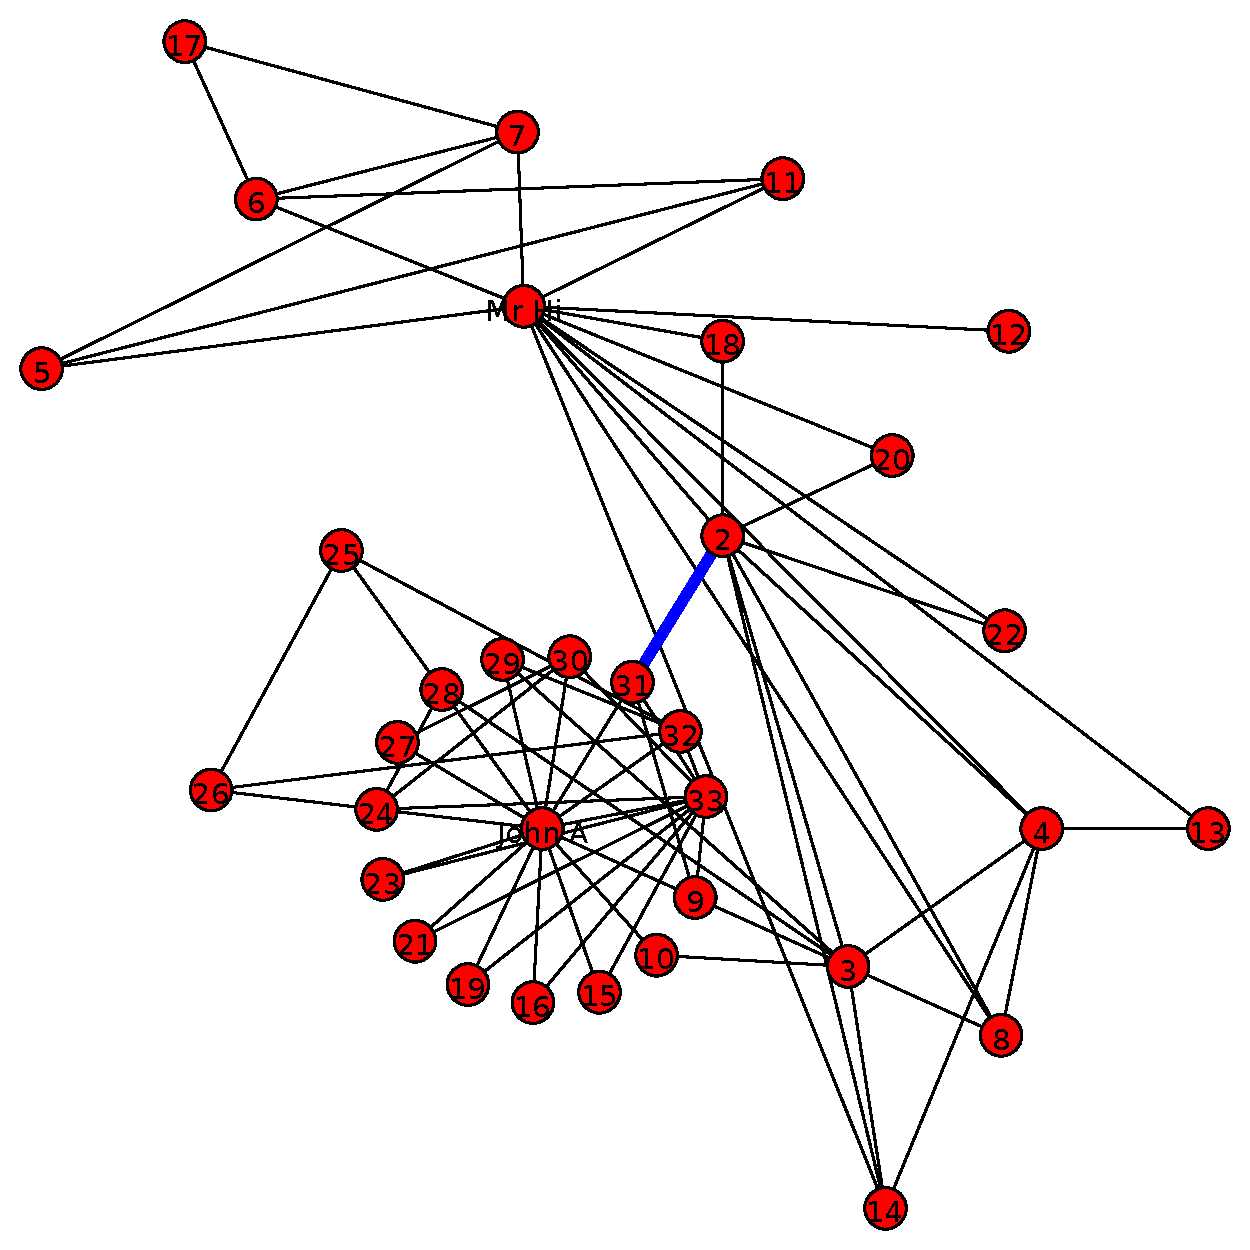
\includegraphics[width=.50\textwidth]{../graphs/sn-6-1.pdf}}
        \subfigure[Iteration: 7, Clusters: 1]{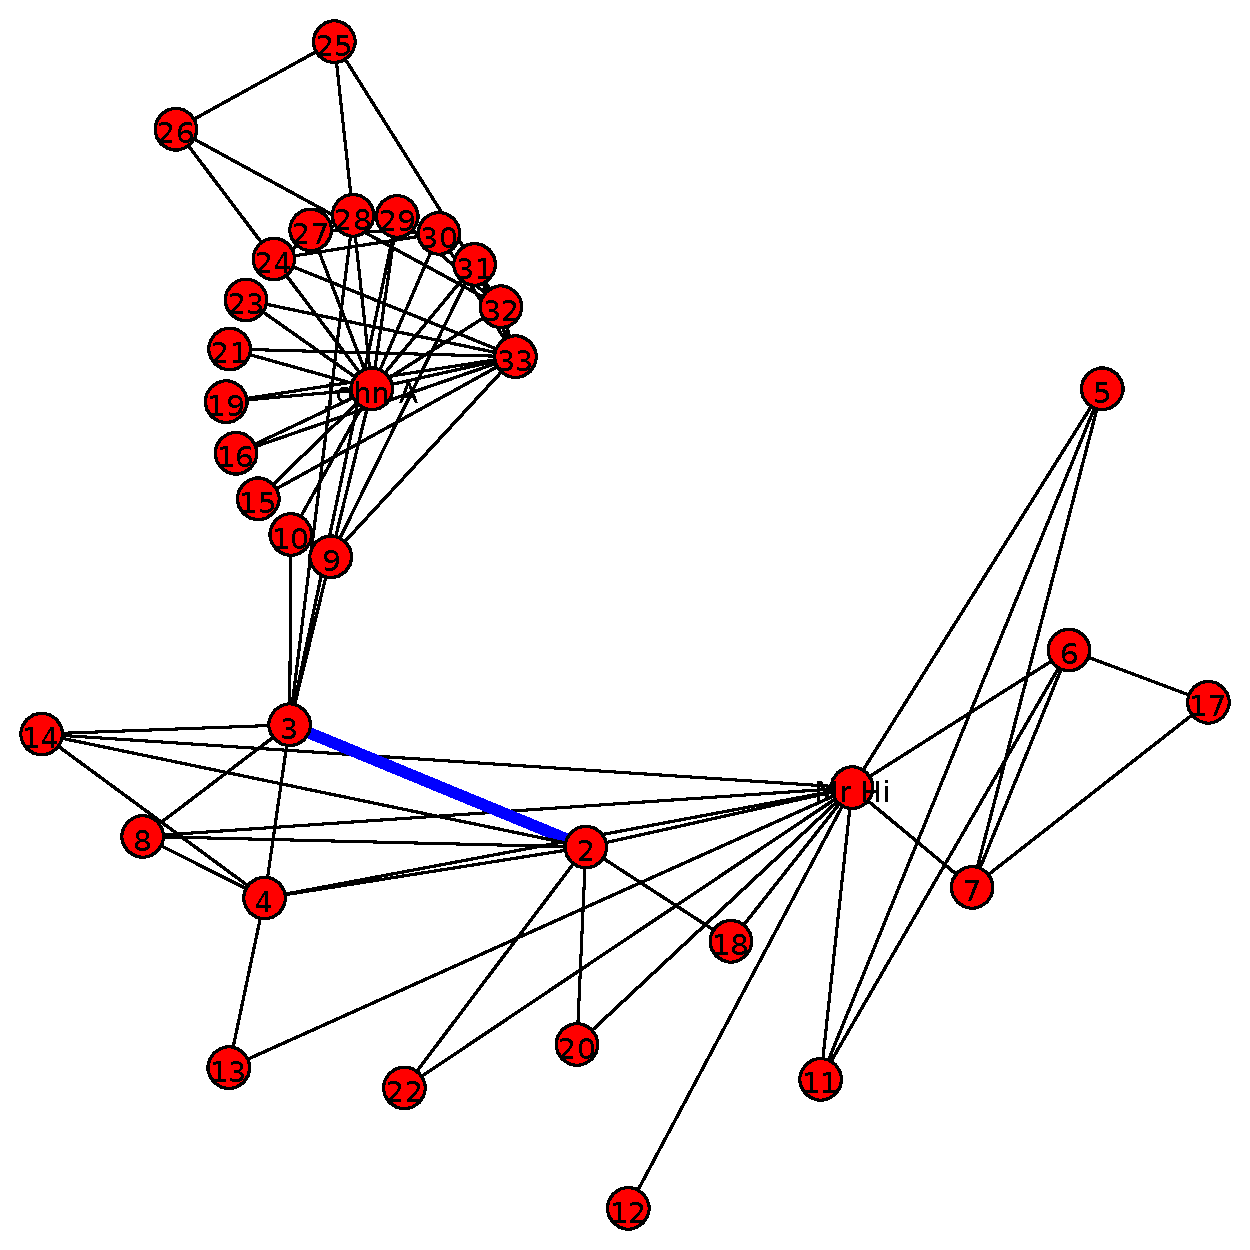
\includegraphics[width=.50\textwidth]{../graphs/sn-7-1.pdf}}

    \end{figure}

    \begin{figure}
        \caption{Multiple Iterations Of The Girvin-Newman Algorithm}
        \subfigure[Iteration: 8, Clusters: 1]{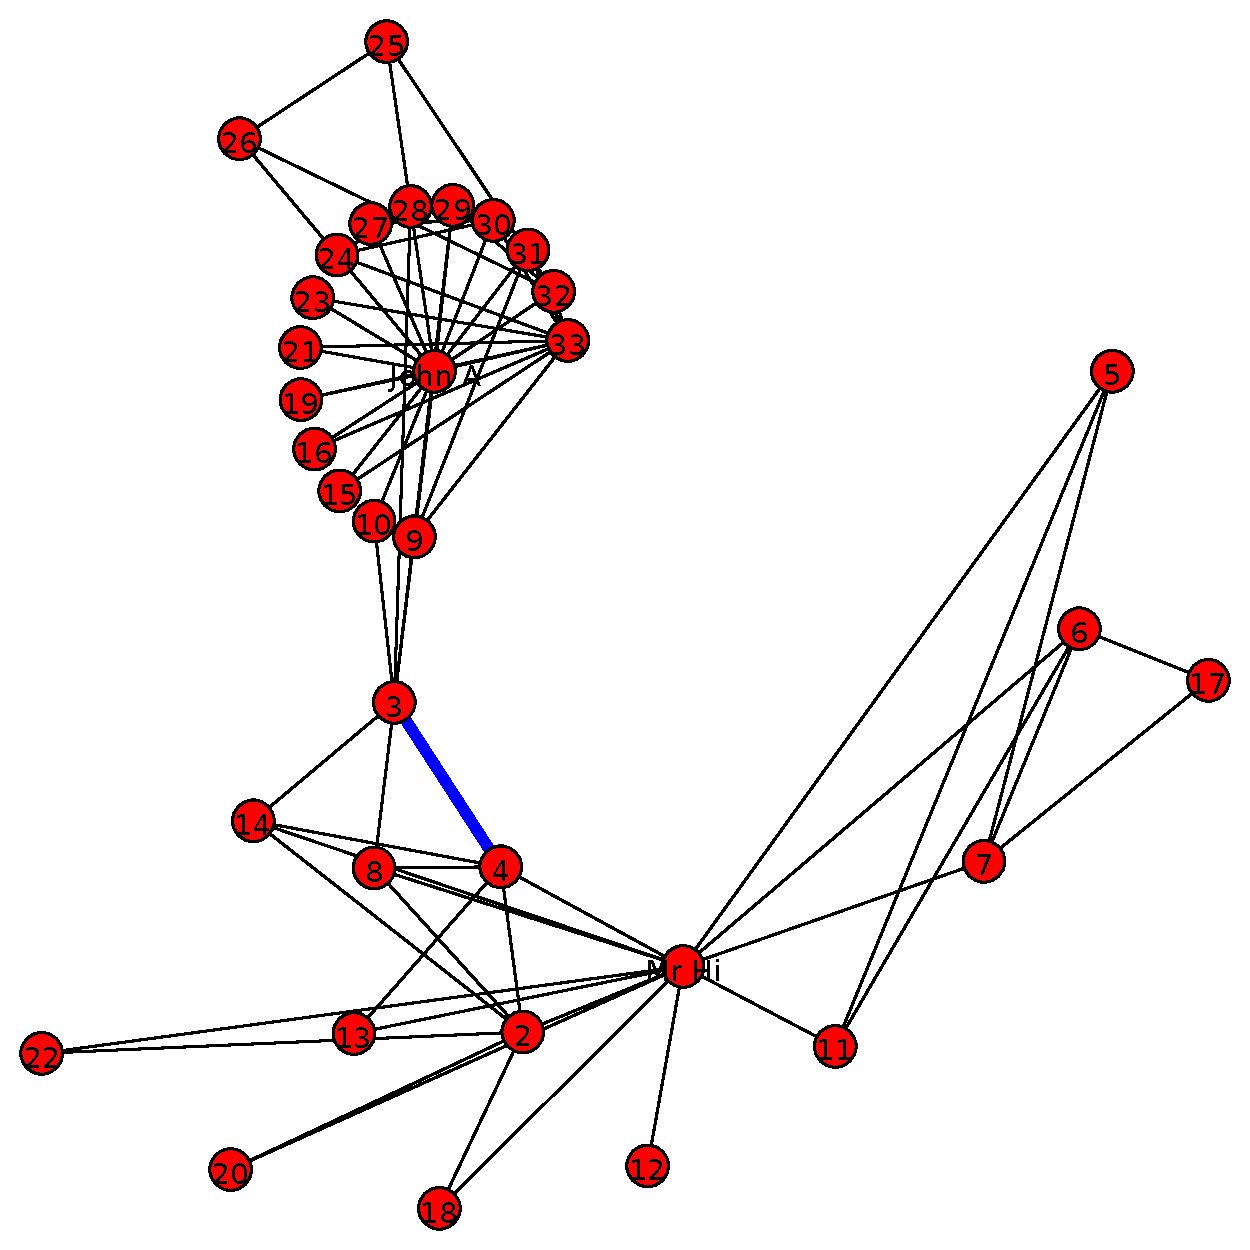
\includegraphics[width=.50\textwidth]{../graphs/sn-8-1.pdf}}
        \subfigure[Iteration: 9, Clusters: 1]{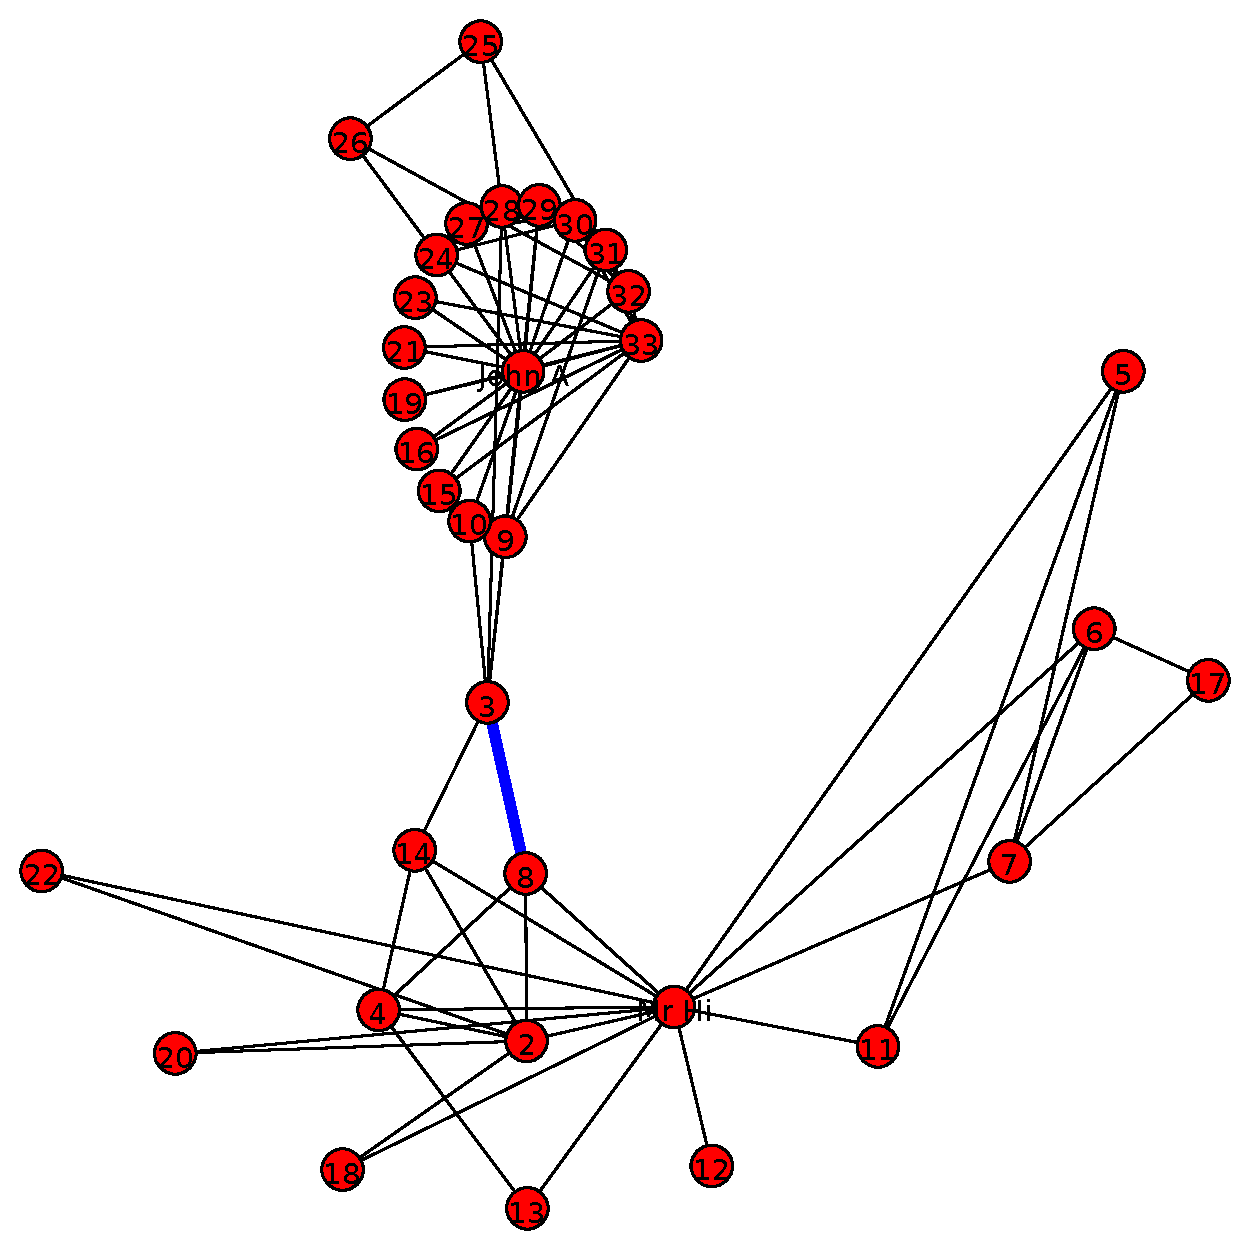
\includegraphics[width=.50\textwidth]{../graphs/sn-9-1.pdf}}
        \subfigure[Iteration: 10, Clusters: 1]{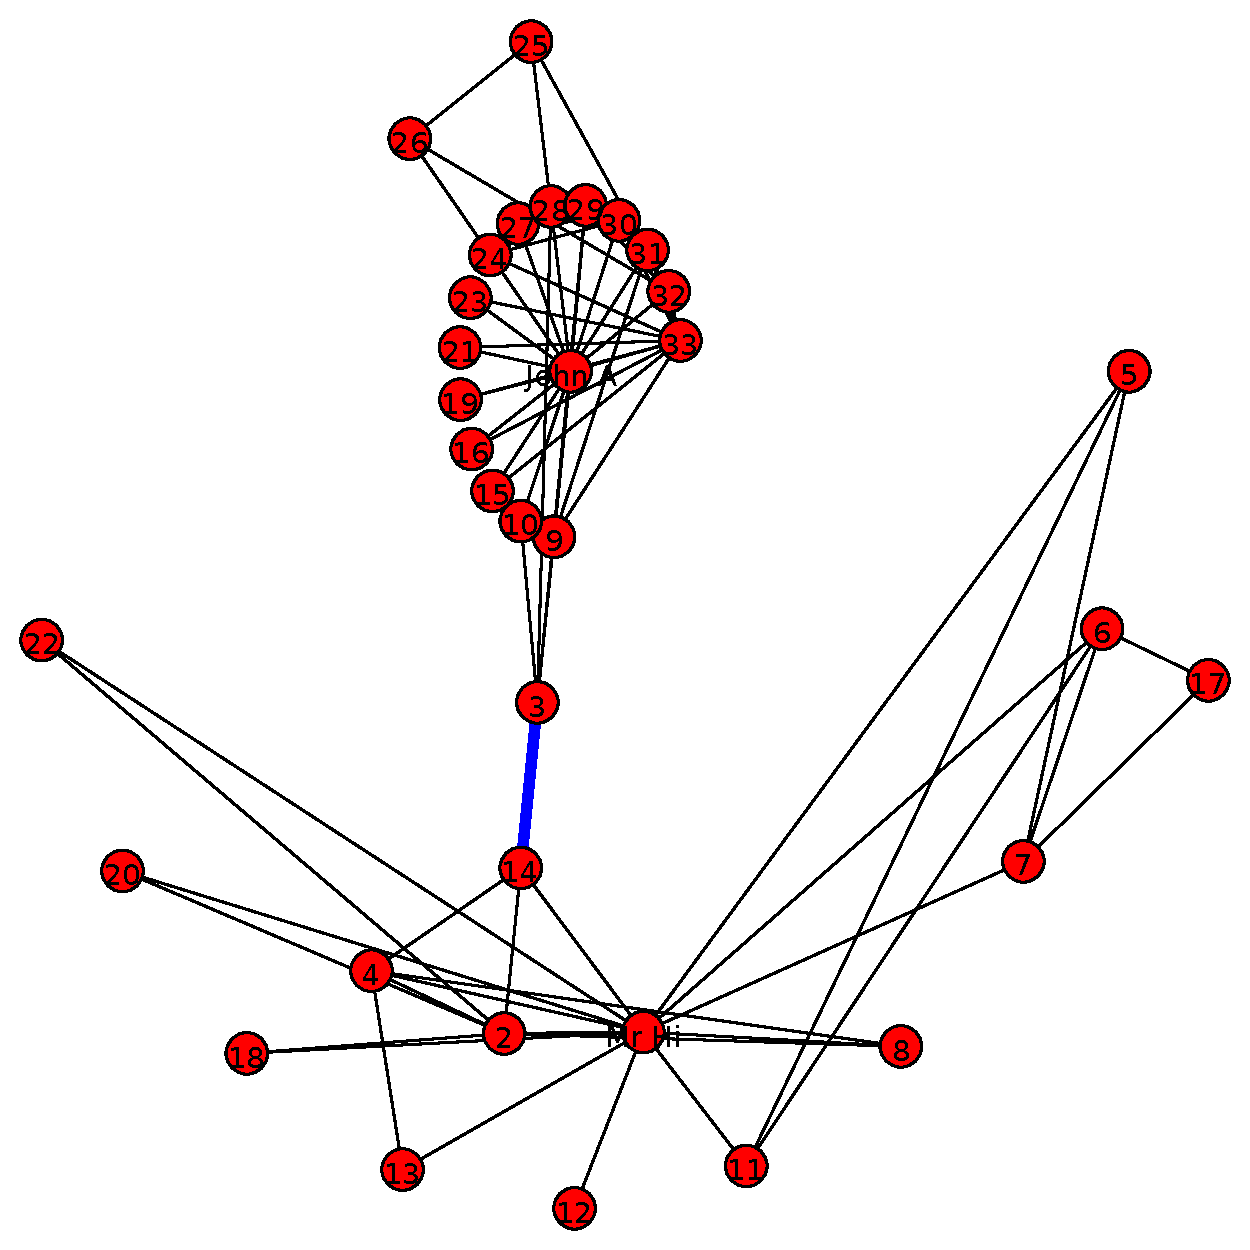
\includegraphics[width=.50\textwidth]{../graphs/sn-10-1.pdf}}
        \subfigure[Iteration: 11, Clusters: 2]{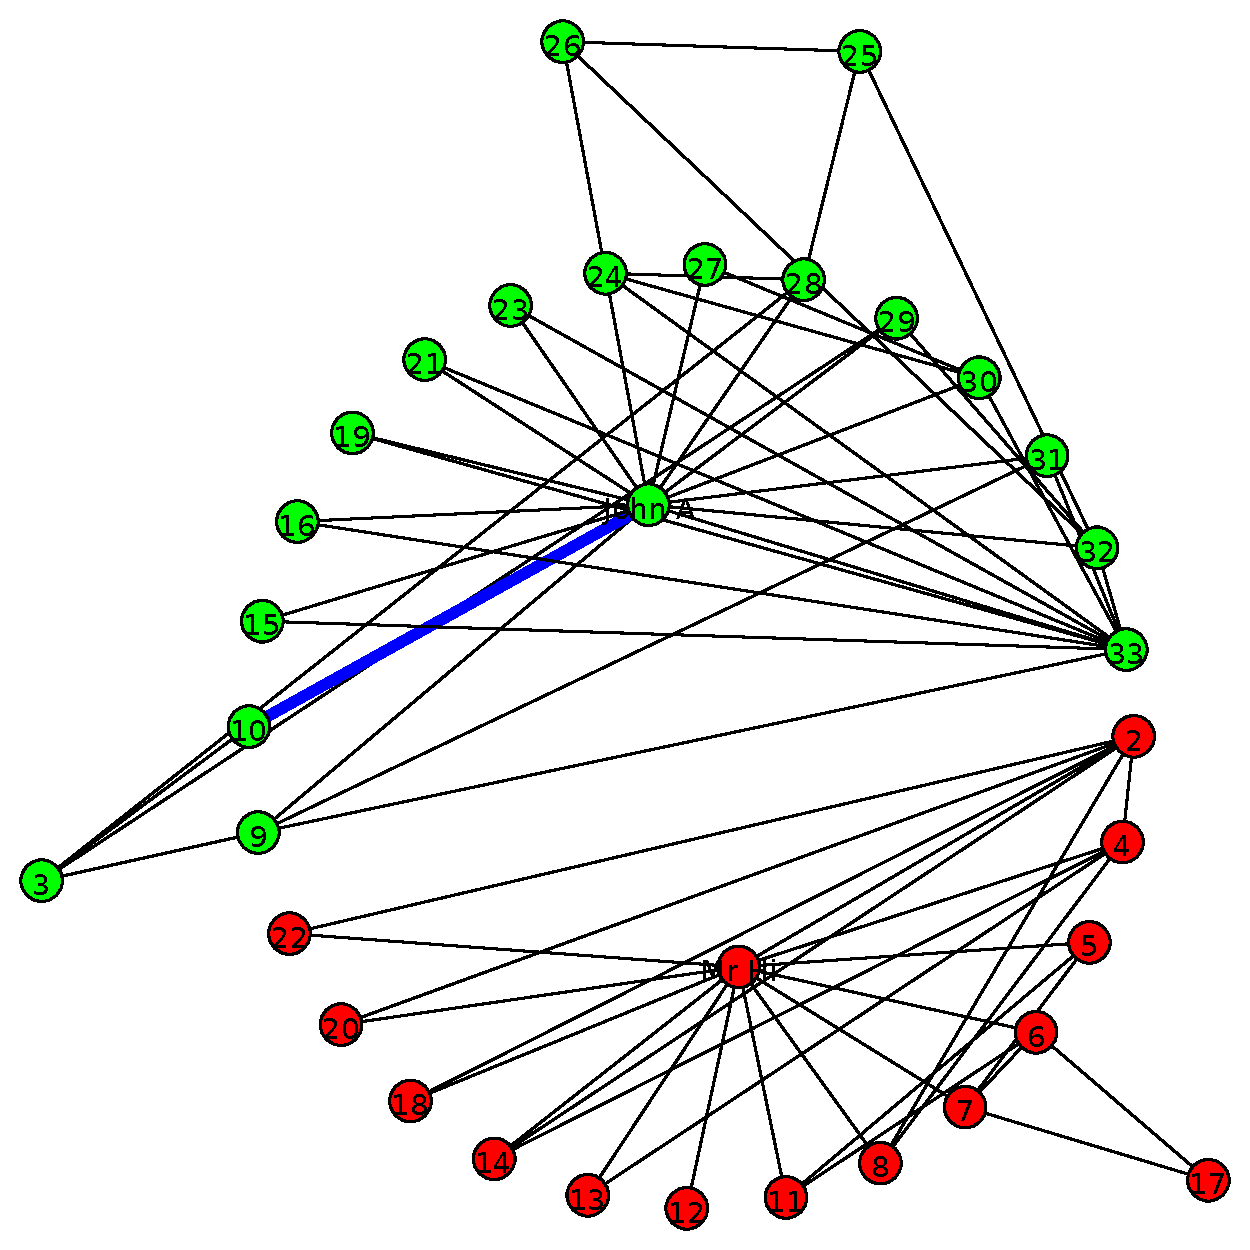
\includegraphics[width=.50\textwidth]{../graphs/sn-11-2.pdf}}
    \end{figure}

    \textbf{CONCLUSION 1}\\

    After the 11th iteration (12th run), as seen in \textbf{Figure 4d}, the graph contains 2 clusters with John A. as the central figure of the first cluster, and Mr. Hi - the second cluster. Let us compare the factions from \textbf{Figure 4d} to the result of the split, \textbf{Figure 1b}. Let us call the original result of the split graph RS and the results of running the Girvin-Newman algorithm GV. As seen below, only 1 descrepancey exists - Node 3. So it is fair to say the Girvin-Newman Algorithm fairly represents reality.

    \begin{verbatim}
    Faction 1:
      SR:  <9, 10, 15, 16, 19, 21, 23, 24, 25, 26, 27, 28, 29, 30, 31, 32, 33>
      GV: 3<9, 10, 15, 16, 19, 21, 23, 24, 25, 26, 27, 28, 29, 30, 31, 32, 33>
    Faction 2:
      SR: <2, 3, 4, 5, 6, 7, 8, 11, 12, 13, 14, 17, 18, 20, 22>
      GV: <2, ., 4, 5, 6, 7, 8, 11, 12, 13, 14, 17, 18, 20, 22> 
    \end{verbatim}

%}



\end{homeworkProblem}

%----------------------------------------------------------------------------------------
%	PROBLEM 2
%----------------------------------------------------------------------------------------
\begin{homeworkProblem}
We know the group split in two different groups.  Suppose the
disagreements in the group were more nuanced -- what would the clubs
look like if they split into groups of 3, 4, and 5?

\begin{verbatim}\end{verbatim}
\textbf{SOLUTION 2}\\

As seen from \textbf{Figure 5c}, we have 3 groups after 14 iterations (15 runs)\\
As seen from \textbf{Figure 6c}, we have 4 groups after 18 iterations (19 runs)\\
As seen from \textbf{Figure 8a}, we have 5 groups after 24 iterations (25 runs)

\begin{figure}[h!]

    \caption{Multiple Iterations Of The Girvin-Newman Algorithm}
    \subfigure[Iteration: 12, Clusters: 2]{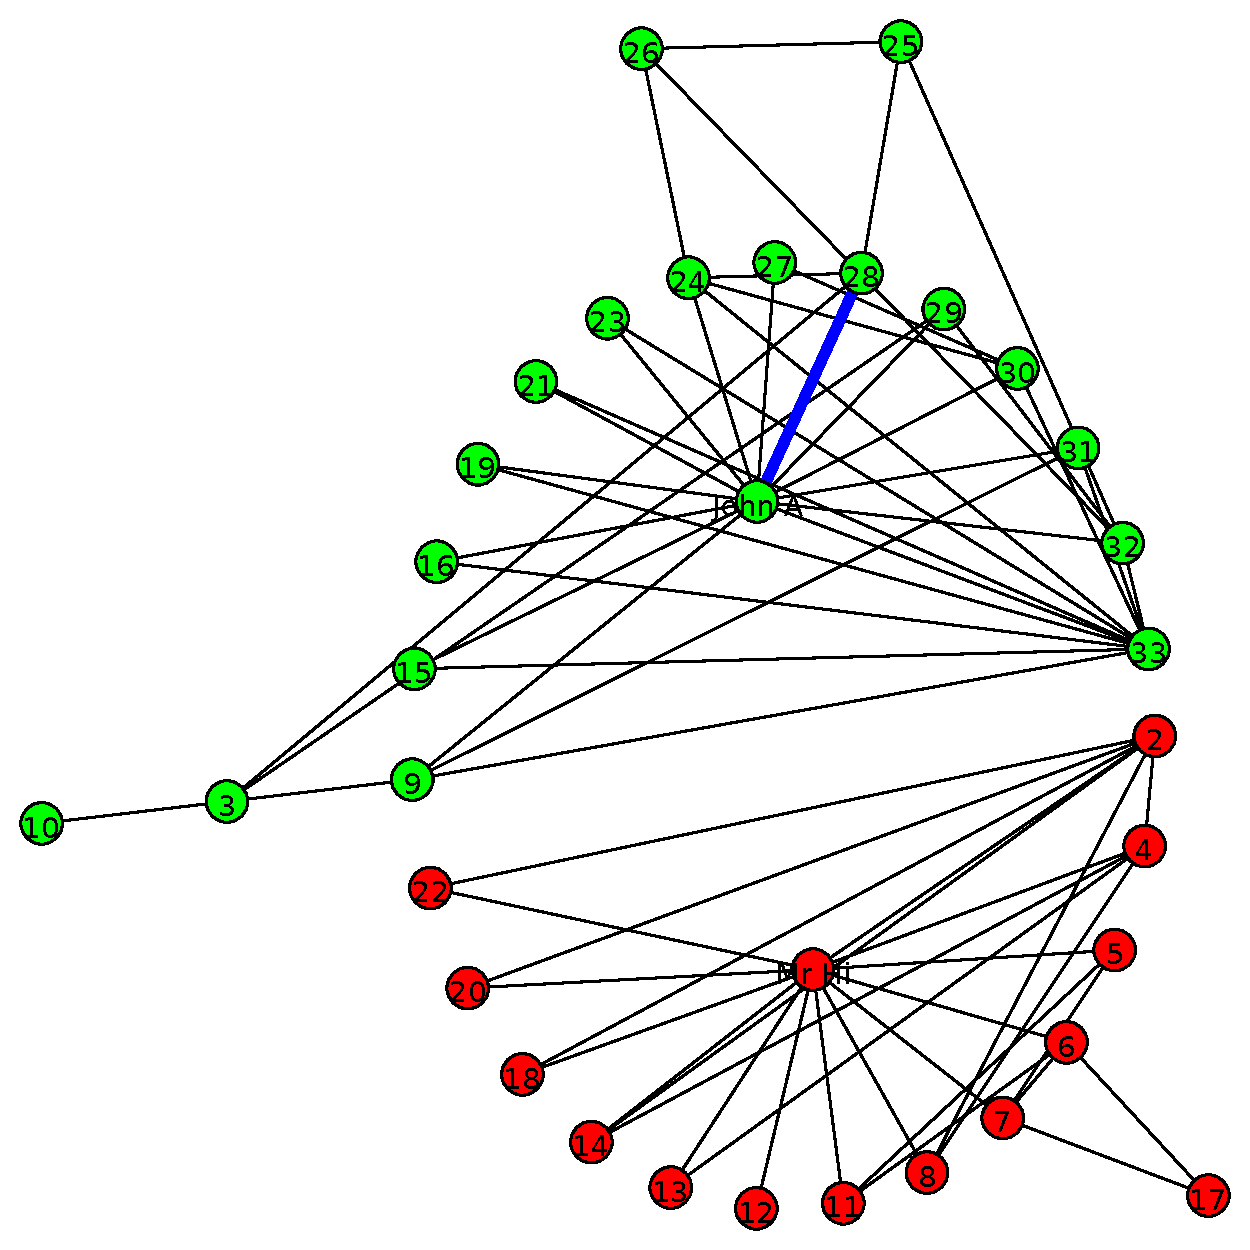
\includegraphics[width=.50\textwidth]{../graphs/sn-12-2.pdf}}
    \subfigure[Iteration: 13, Clusters: 2]{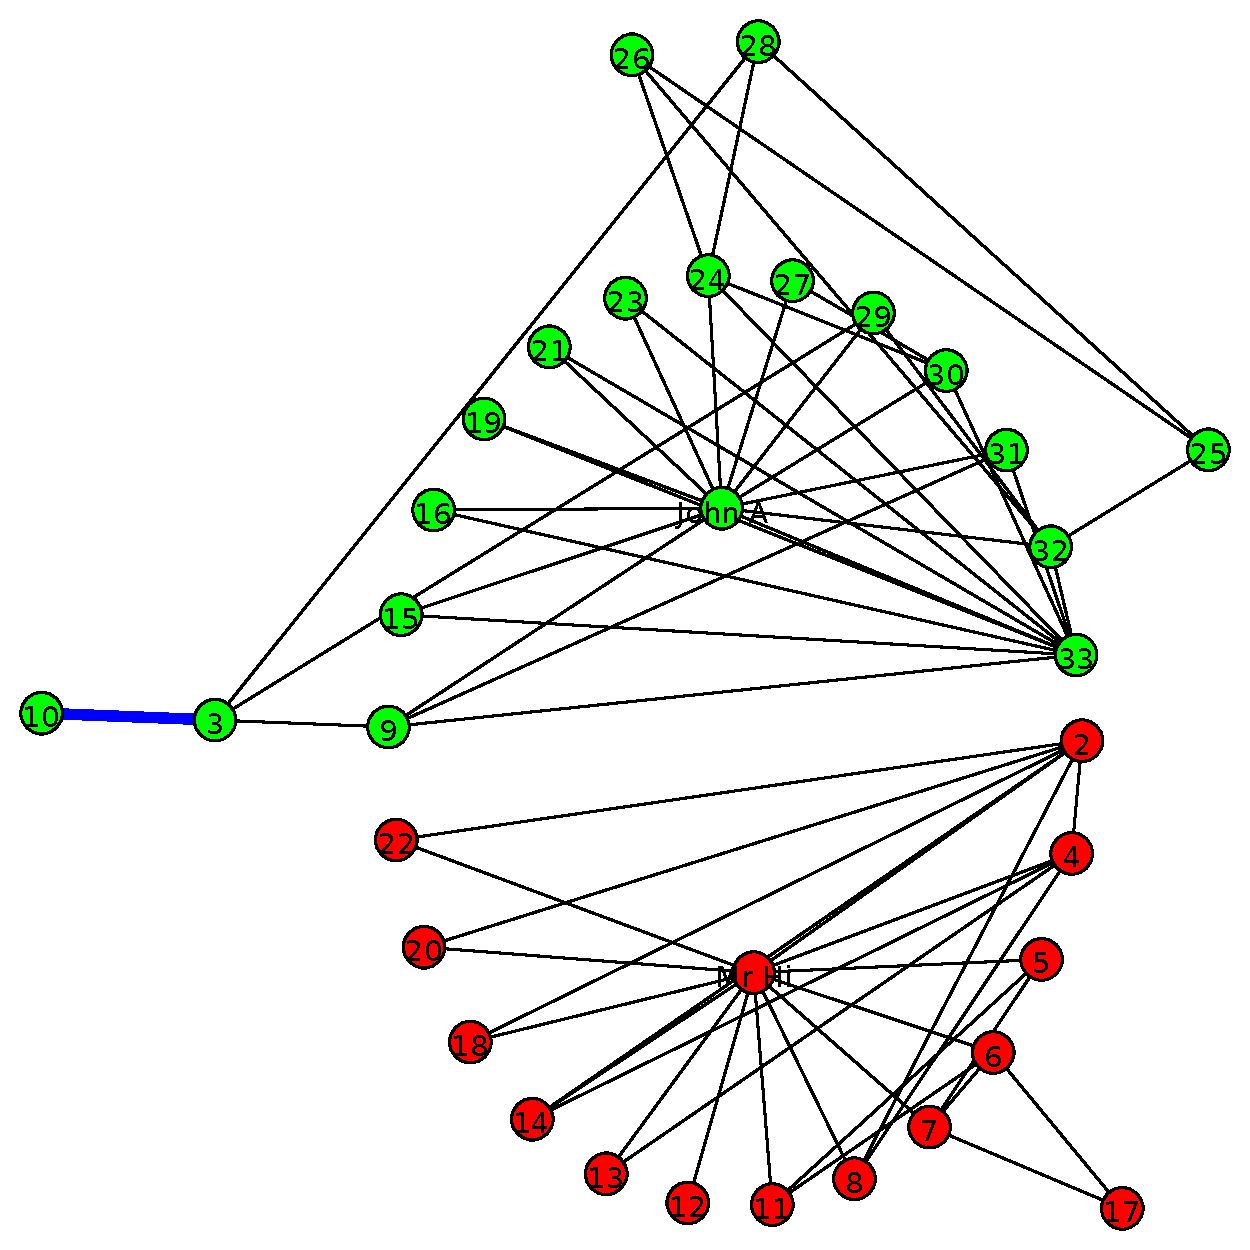
\includegraphics[width=.50\textwidth]{../graphs/sn-13-2.pdf}}
    \subfigure[Iteration: 14, Clusters: 3]{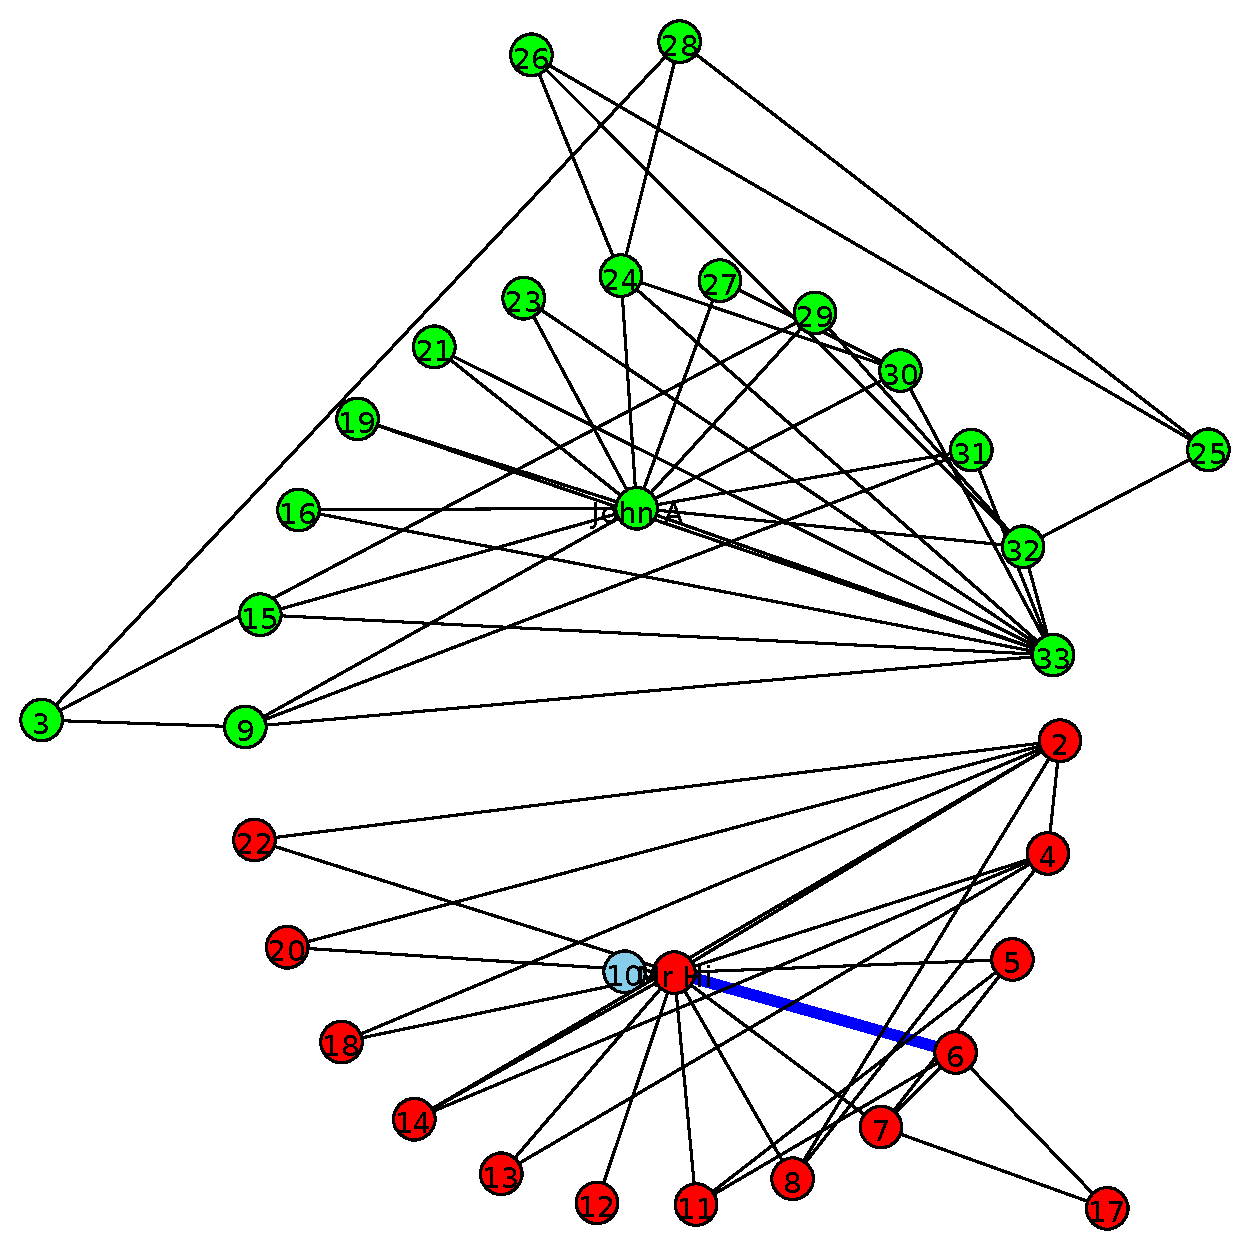
\includegraphics[width=.50\textwidth]{../graphs/sn-14-3.pdf}}
    \subfigure[Iteration: 15, Clusters: 3]{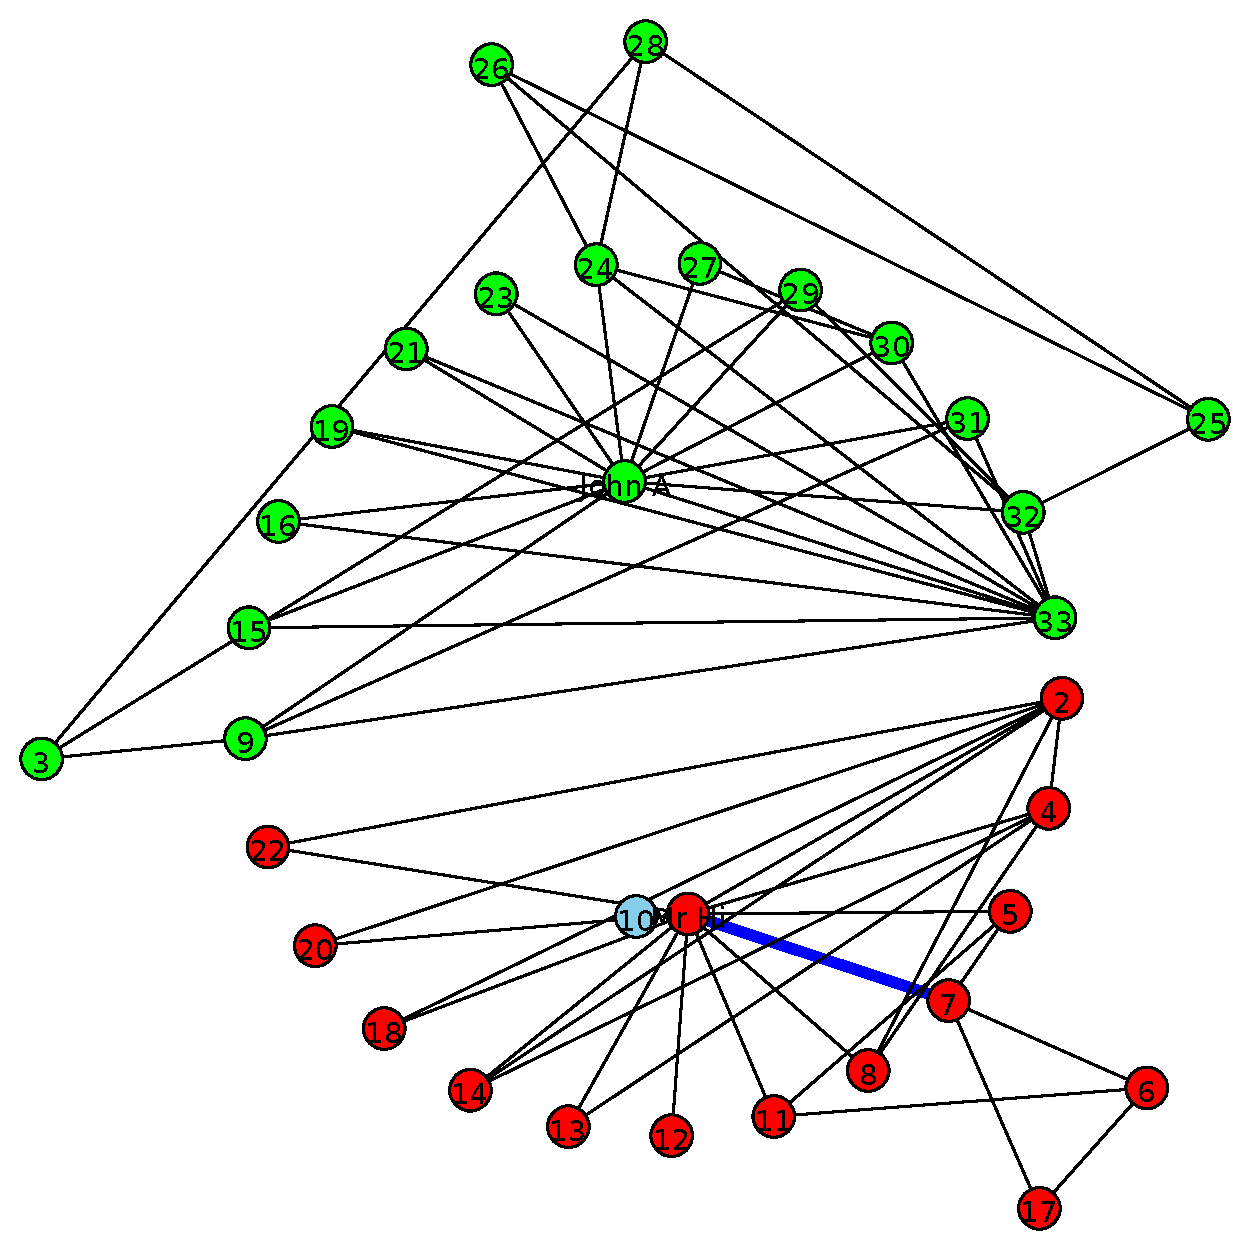
\includegraphics[width=.50\textwidth]{../graphs/sn-15-3.pdf}}

\end{figure}

\begin{figure}

    \caption{Multiple Iterations Of The Girvin-Newman Algorithm}
    \subfigure[Iteration: 16, Clusters: 3]{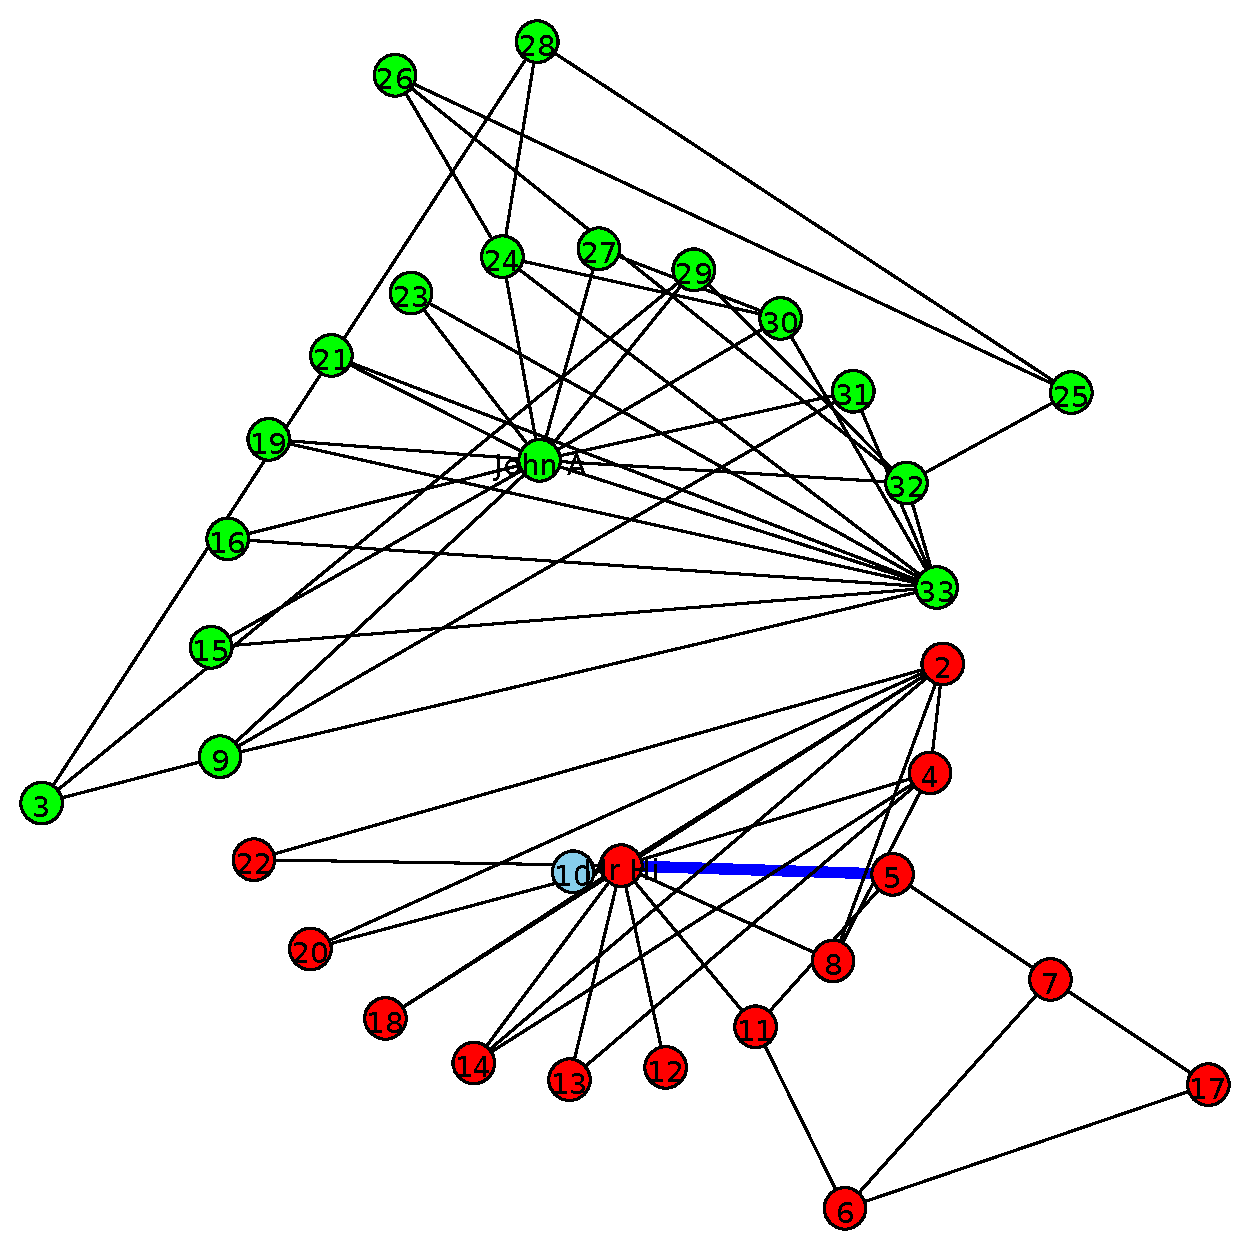
\includegraphics[width=.50\textwidth]{../graphs/sn-16-3.pdf}}
    \subfigure[Iteration: 17, Clusters: 3]{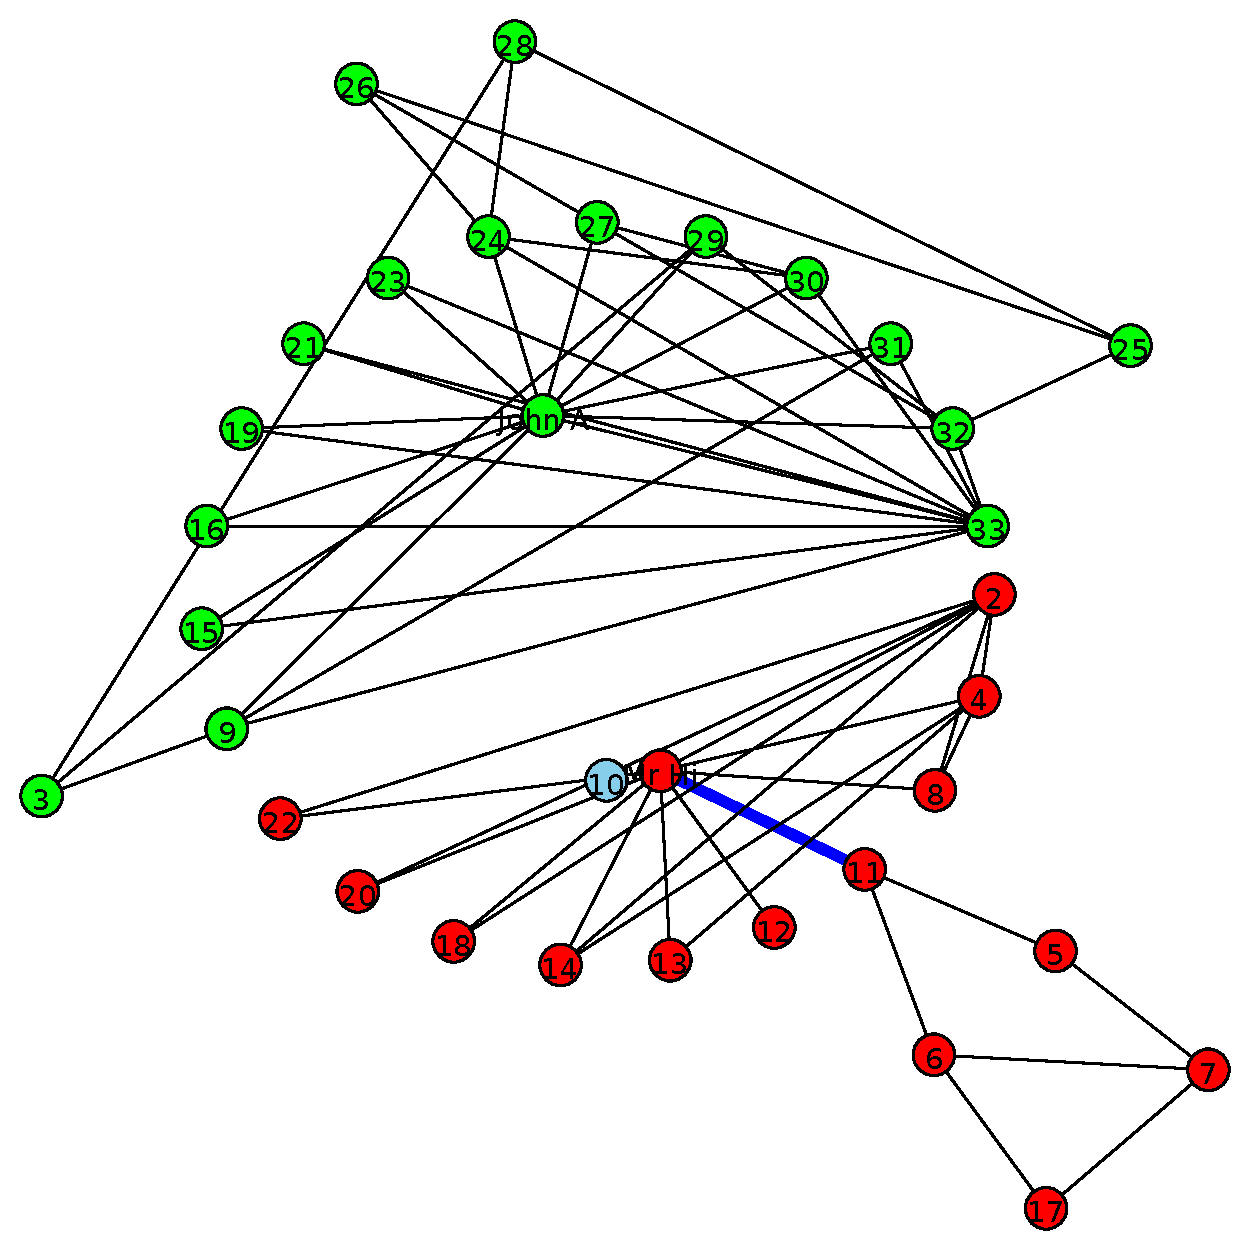
\includegraphics[width=.50\textwidth]{../graphs/sn-17-3.pdf}}
    \subfigure[Iteration: 18, Clusters: 4]{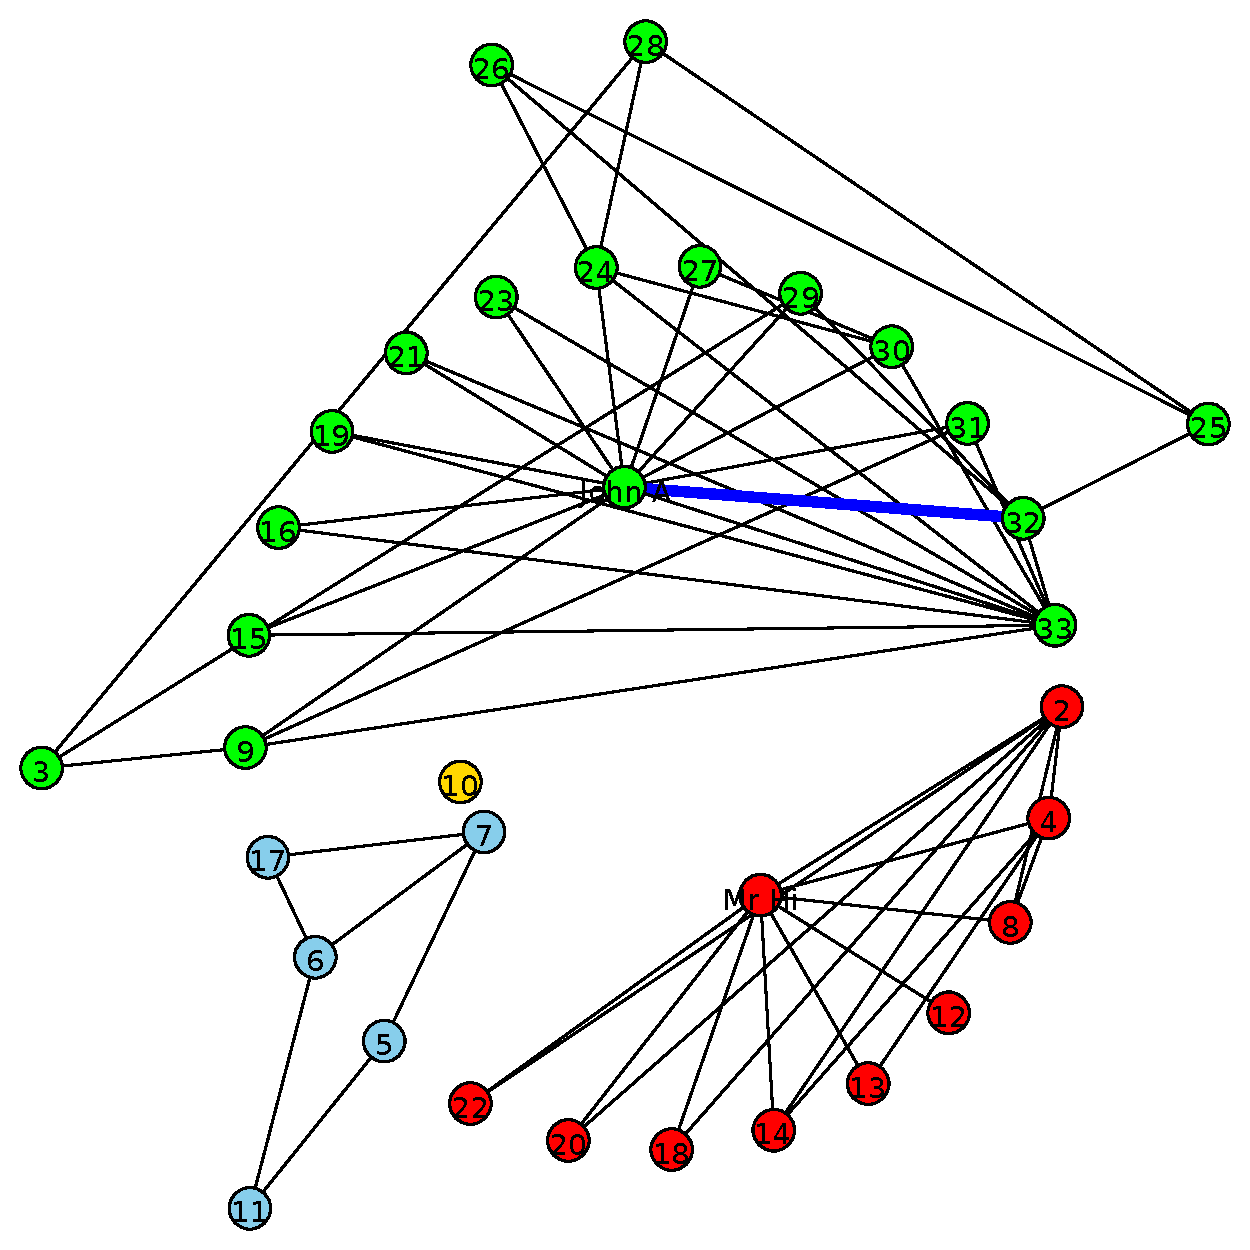
\includegraphics[width=.50\textwidth]{../graphs/sn-18-4.pdf}}
    \subfigure[Iteration: 19, Clusters: 4]{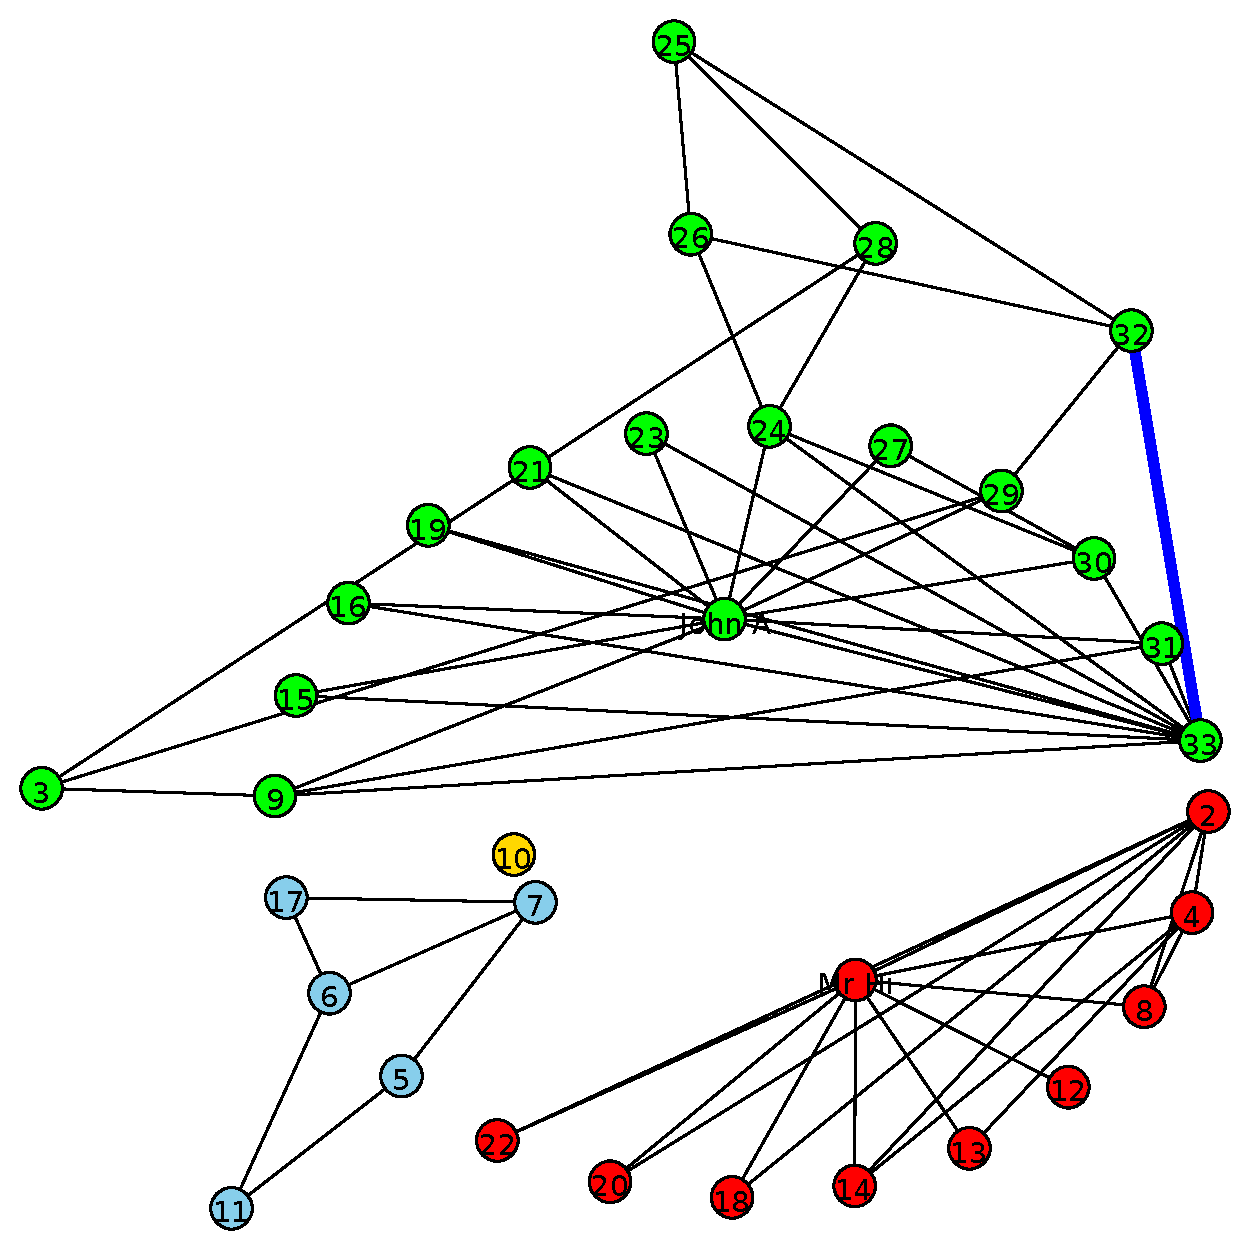
\includegraphics[width=.50\textwidth]{../graphs/sn-19-4.pdf}}

\end{figure}

\begin{figure}

    \caption{Multiple Iterations Of The Girvin-Newman Algorithm}
    \subfigure[Iteration: 20, Clusters: 4]{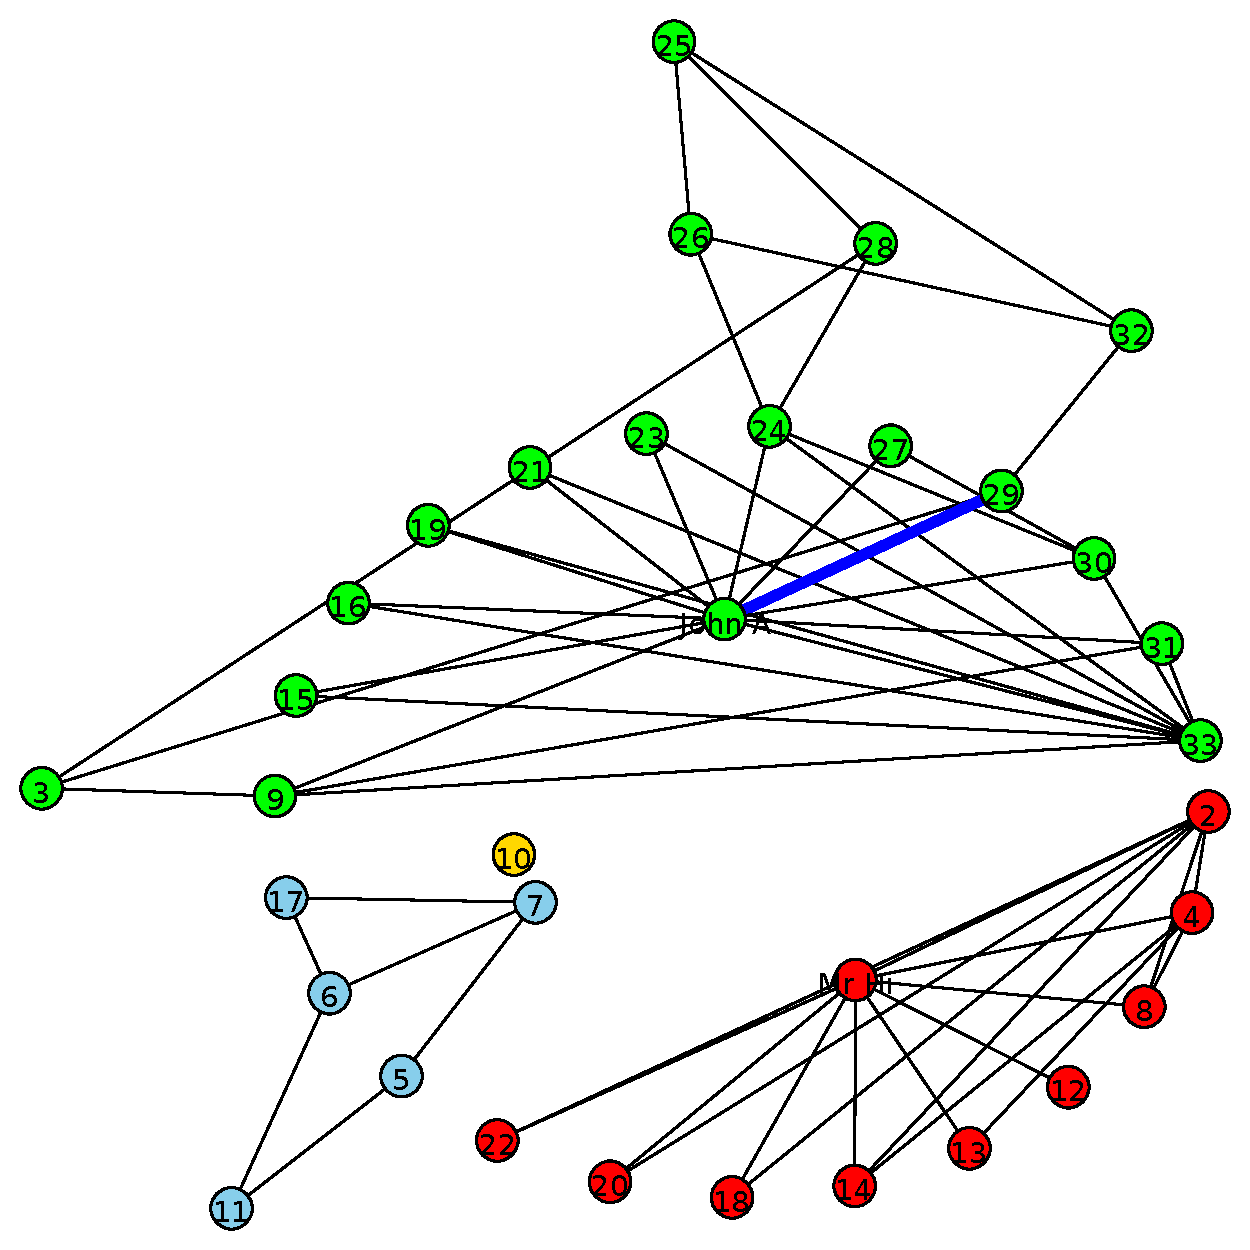
\includegraphics[width=.50\textwidth]{../graphs/sn-20-4.pdf}}
    \subfigure[Iteration: 21, Clusters: 4]{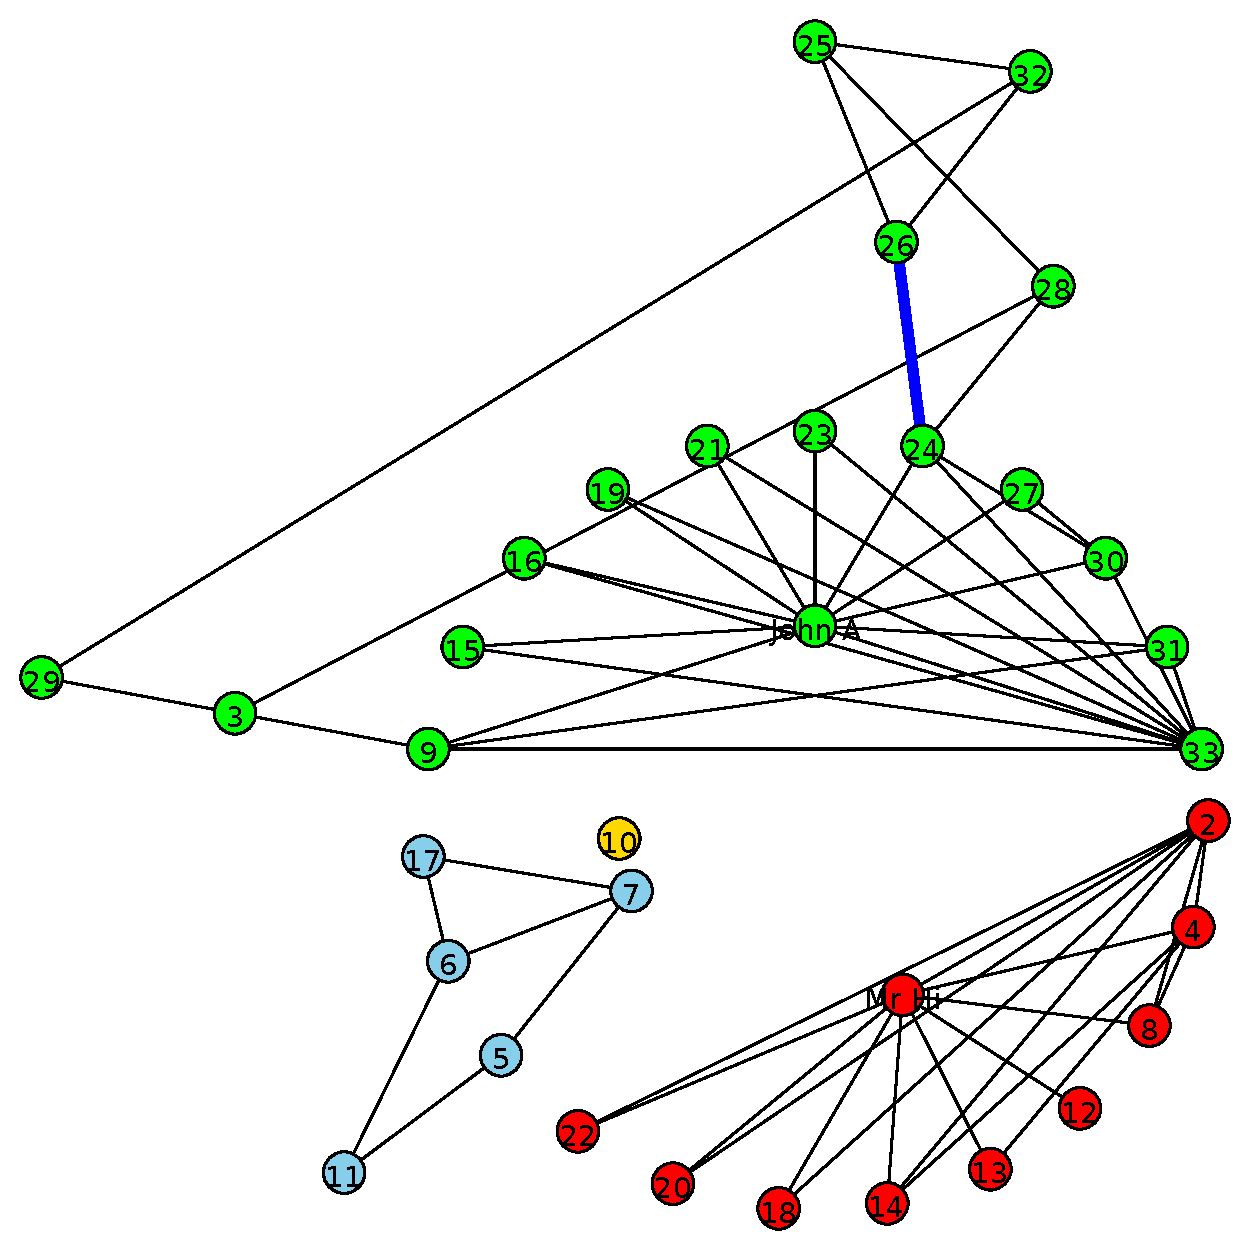
\includegraphics[width=.50\textwidth]{../graphs/sn-21-4.pdf}}
    \subfigure[Iteration: 22, Clusters: 4]{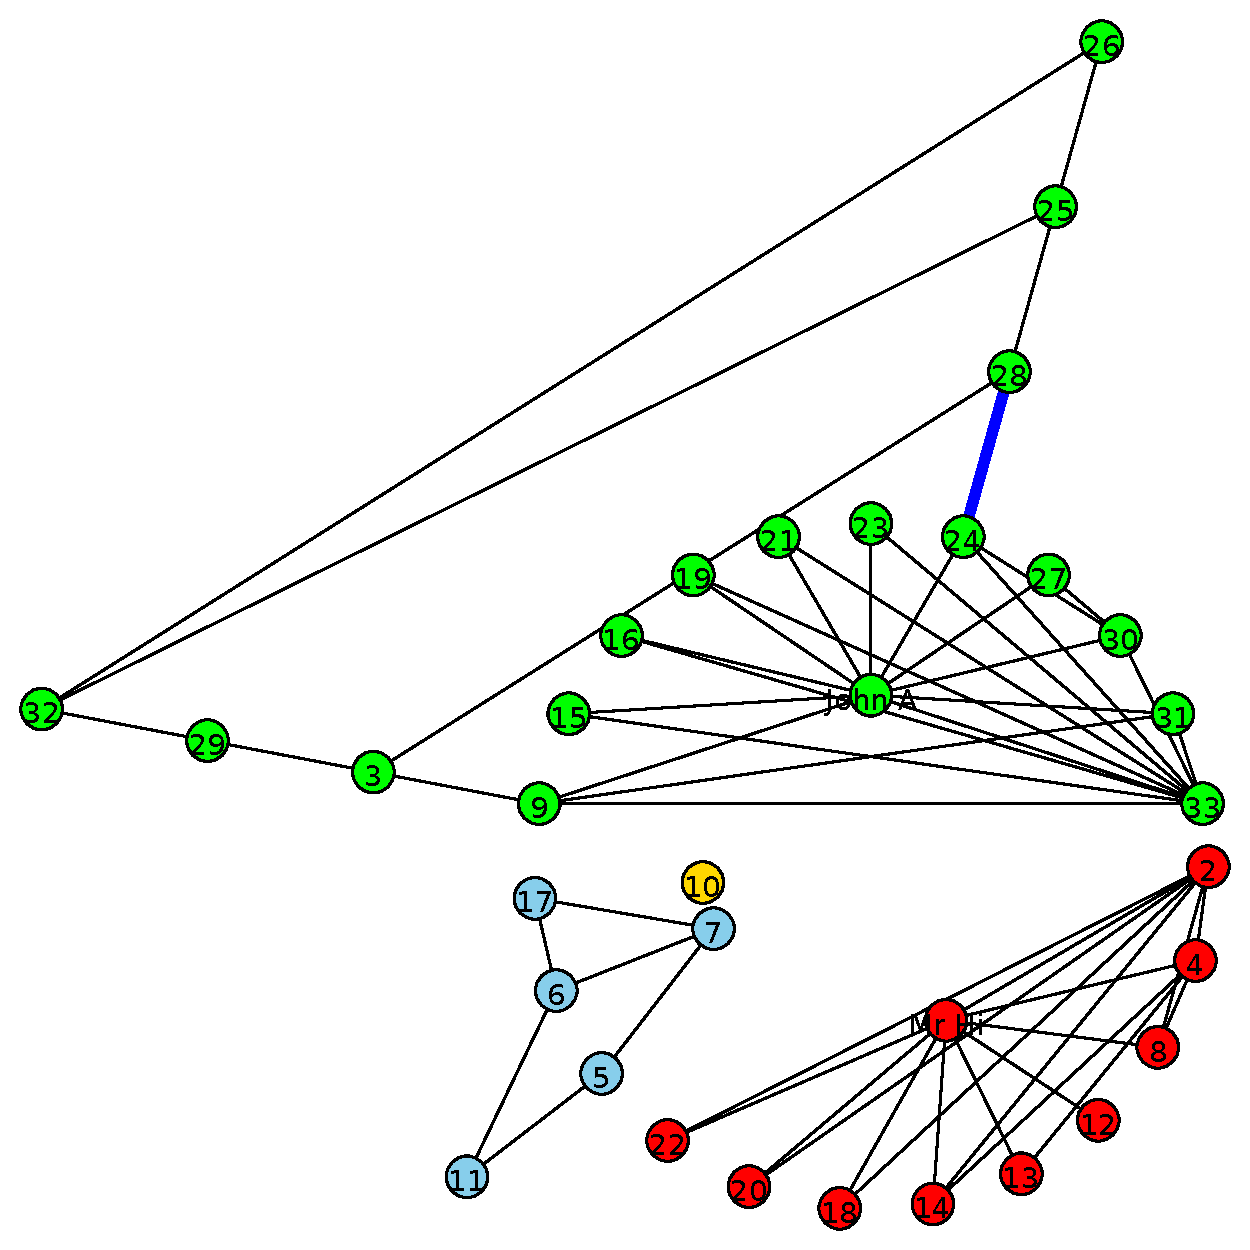
\includegraphics[width=.50\textwidth]{../graphs/sn-22-4.pdf}}
    \subfigure[Iteration: 23, Clusters: 4]{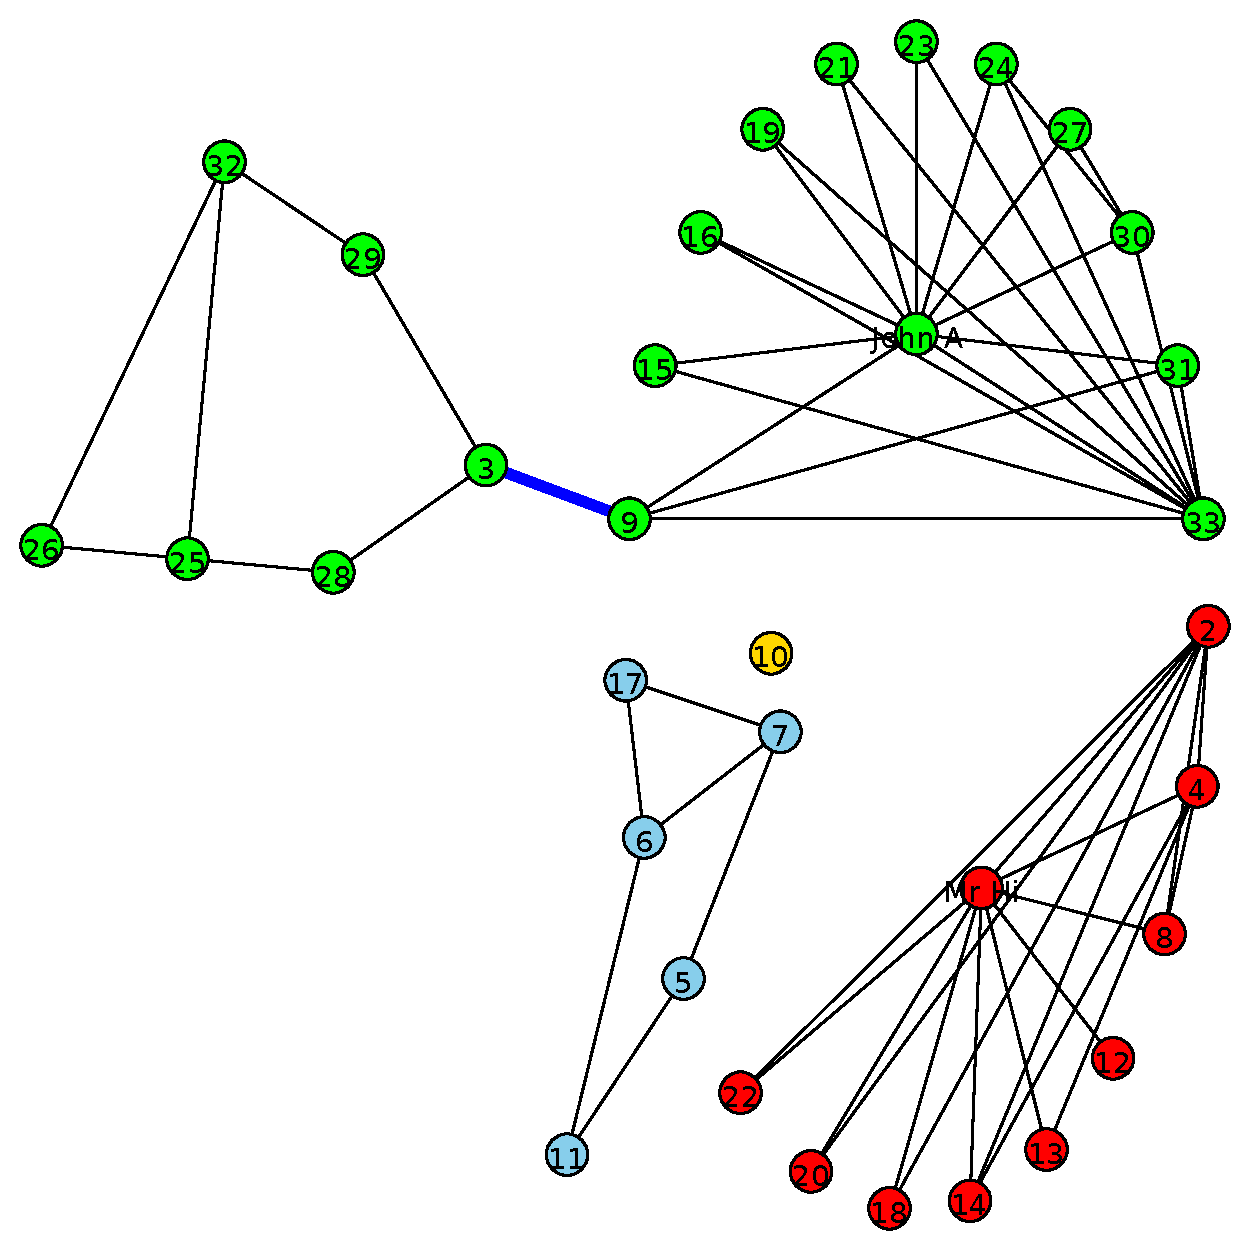
\includegraphics[width=.50\textwidth]{../graphs/sn-23-4.pdf}}

\end{figure}

\begin{figure}

    \caption{Multiple Iterations Of The Girvin-Newman Algorithm}
    \subfigure[Iteration: 24, Clusters: 5]{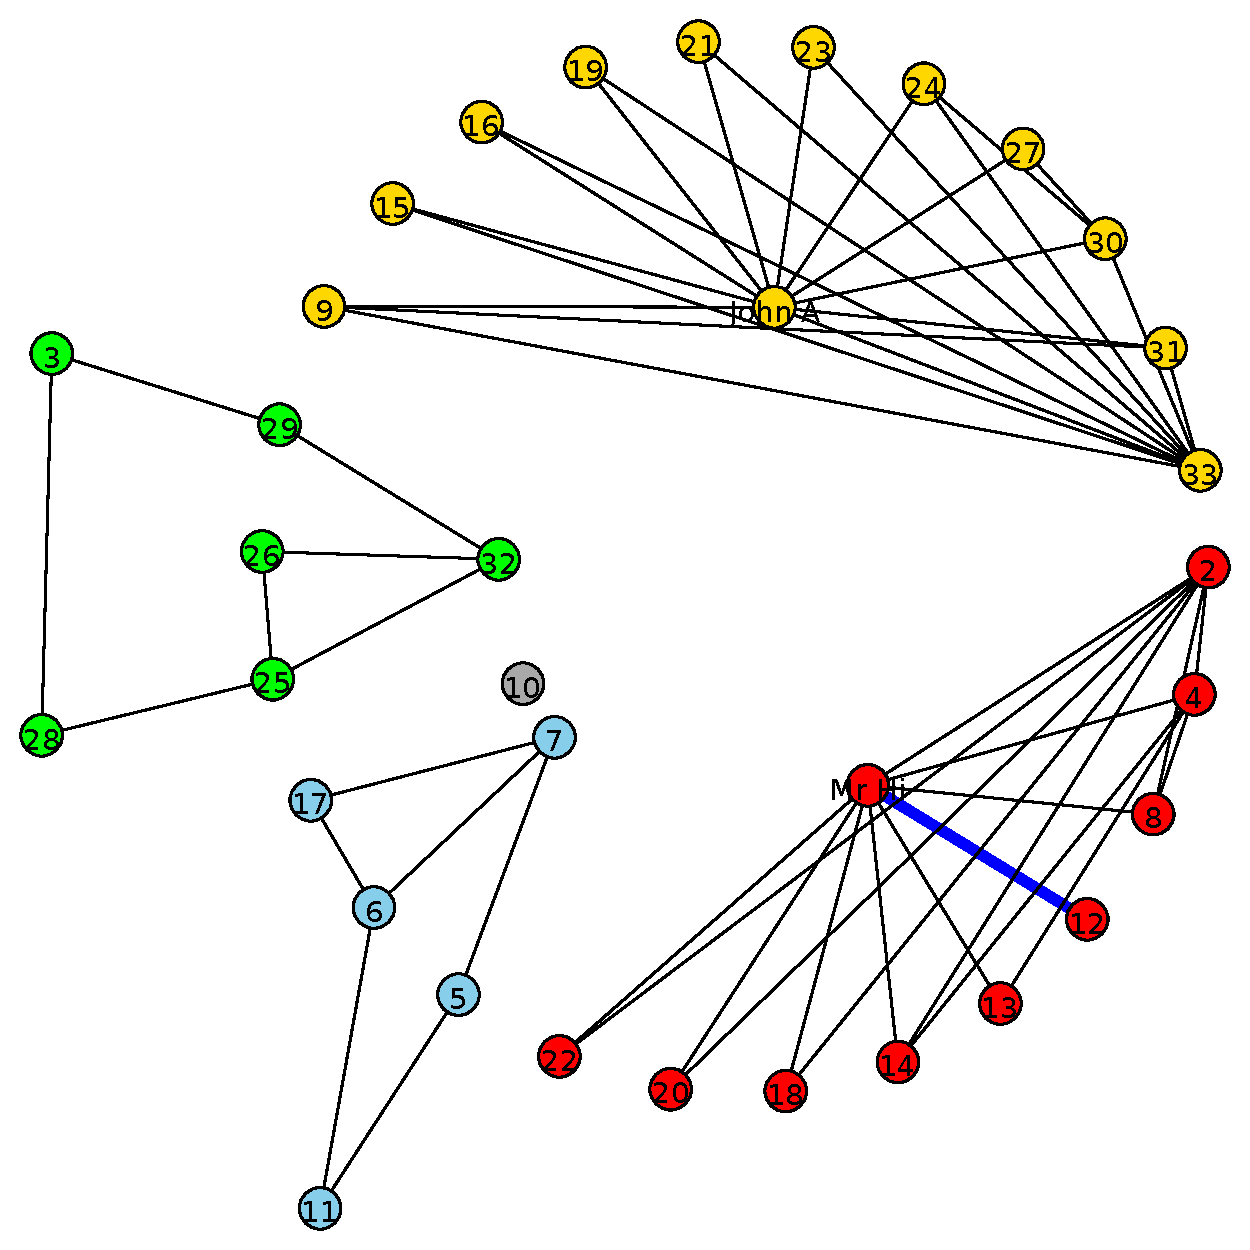
\includegraphics[width=\textwidth]{../graphs/sn-24-5.pdf}}

\end{figure}

\end{homeworkProblem}

\bibliographystyle{plain}
\bibliography{A6bibFile}

%----------------------------------------------------------------------------------------

\end{document}